%%%%%%%%%%%%%%%%%%%%%%%%%%%%%%%%%%%%%%%%%%%%%%%%%%%%%%%%%%%%%%%%%%%%%%%%%%
%% Trim Size: 9.75in x 6.5in
%% Text Area: 8in (include Runningheads) x 5in
%% ws-ijhr.tex   :  9-5-2005 
%% Tex file to use with ws-ijhr.cls written in Latex2E.
%% The content, structure, format and layout of this style file is the
%% property of World Scientific Publishing Co. Pte. Ltd.
%% Copyright 1995, 2003 by World Scientific Publishing Co.
%% All rights are reserved.
%%%%%%%%%%%%%%%%%%%%%%%%%%%%%%%%%%%%%%%%%%%%%%%%%%%%%%%%%%%%%%%%%%%%%%%%%%%%
%

%%%%%%%%%%%%% FOR TEMPLATE OF TYPING OUT THE BIBLIOGRAPHY TEXT ONLY %%%%%%%%
%\newcounter{myctr}
%\def\myitem{\refstepcounter{myctr}\bibfont\parindent0pt\hangindent13pt\themyctr.\enskip}
%\def\myhead#1{\vskip10pt\noindent{\bibfont #1:}\vskip4pt}
%%%%%%%%%%%%% FOR TEMPLATE OF TYPING OUT THE BIBLIOGRAPHY TEXT ONLY %%%%%%%%

\documentclass{ws-ijhr}

\usepackage{graphicx}
\graphicspath{ {./img/} {../img/} }
\usepackage{multirow}
\usepackage{colortbl}
\usepackage{booktabs}
\usepackage[algoruled,vlined]{algorithm2e}
\usepackage{amsmath,amsfonts,amssymb,amsxtra,amsbsy,amsopn}
\usepackage{paralist}
\usepackage{booktabs}
\usepackage{tabularx}
% argmax as math operator
\DeclareMathOperator*{\argmax}{arg\,max}

% todonotes, pass disable as option to also remove all notes
\usepackage[textsize=tiny]{todonotes}


\begin{document}

\markboth{Rosales et al.}{GPAtlasRRT: A local tactile exploration planner}

%%%%%%%%%%%%%%%%%%%%% Publisher's Area please ignore %%%%%%%%%%%%%%%
%
\catchline{}{}{}{}{}
%
%%%%%%%%%%%%%%%%%%%%%%%%%%%%%%%%%%%%%%%%%%%%%%%%%%%%%%%%%%%%%%%%%%%%

\title{GPAtlasRRT: A local tactile exploration planner for recovering the shape of novel objects.
  \thanks{This work is supported by EC-FP7-ICT-600918, PacMan.}}

\author{Carlos Rosales, Federico Spinelli, Marco Gabiccini\footnote{Universita di Pisa.}}

\address{Centro di Ricerca E. Piaggio, Univ. di Pisa, Pisa, Italy.\\
carlos.rosales@for.unipi.it}

\author{Claudio Zito, Jeremy L. Wyatt}

\address{IRLab, CN-CR, School of Computer Science\\
University of Birmingham, Birmingham, B15 2TT, UK\\
\{C.Zito, J.L.Wyatt\}@cs.bham.ac.uk}

\maketitle

\begin{history}
\received{1 April 2017} %
\revised{26 November 2017}  %
\accepted{15 January 2018} %
%\comby{(xxxxxxxxxx)}
\end{history}

\begin{abstract}
Touch is an important modality to recover object shape. We present a method for a robot to complete a partial shape model by {\em local tactile exploration}.  In local tactile exploration the finger is constrained to follow the local surface. This is useful for recovering information about a contiguous portion of the object and is frequently employed by humans. There are three contributions. First, we show how to segment an initial point cloud of a grasped, unknown object into hand and object. Second, we present a local tactile exploration planner. This combines a Gaussian Process (GP) model of the object surface with an AtlasRRT planner. The GP predicts the unexplored surface and the uncertainty of that prediction. The AtlasRRT creates a {\em tactile exploration path} across this predicted surface, driving it towards the region of greatest uncertainty. Finally, we experimentally compare the planner with alternatives in simulation, and demonstrate the complete approach on a real robot. We show that our planner successfully traverses the object, and that the full object shape can be recovered with a good degree of accuracy.


\keywords{Shape modeling; Tactile exploration}
\end{abstract}

%%%%%%%%%%%%%%%%%%%%%%%%%%%%%%%%%%%%%%%%%%%%%%%%%%%%%%%%%%%%%%%%%%%%%%%%%%%%%%%%
\section{Introduction}
\label{sec:intro}


% why the problem we are dealing with is important
One of the main reasons that makes autonomous grasping tasks very challenging is that object properties required for grasp planning like shape and surface properties are not known \emph{a priori}. This requires robots to perceive objects around them based on sesnory information.

$ 8< ---- 8< ---- 8< ---- 8< ---- $

% why tactile exploration is not so developed
% and what makes the problem harder that active vision

% why we propose touch (Bajcsy) and why ITS

% what is exactly our contribution

% RELATED WORK

% only localization

% also shape reconstruction
% they also use GP

% what are we doing more at least in surface exploration?
% we are exploiting the implicit manifold nature of GP representation
% and adapt efficient sample-based method for exploring the manifold in
% an intrinsic  way.  

 

General guidelines : \citet{Bajcsy1989Machine}

Active visual perception: \citet{Bajcsy1988Active}

Vision-based exploration is the most studied, perhaps due to its non-invasive nature, which avoids the contact between rigid bodies which is the cause of most headaches in physics modelling, simulation and control.

As very well said by \citet{Petrovskaya2011Global}, even when initial works date back to the 80's, tactile perception has not been addressed as deeply as the non-invasive counterpart, visual perception. Besides the need of being actively controlled, tactile sensors typically required ad-hoc mechanical devices.

``Touch-based perception has not been studied in as much depth
as vision because standardized touch sensors are not as easily
available. In many situations, tactile sensors have to be hand
crafted specifically for the robot and the task. This complicates
comparisons between methods and slows progress in tactile
perception. However, recently there has been a surge of interest
in the field due to the necessity of touch-based perception in
service applications''

Whereas \citet{Petrovskaya2011Global} is more interested in the object pose estimation problem, here we are more interested in the object shape modelling, sort of in the mapping of rather than localization in a SLAM problem.

On active touch sensing \citet{Prescott2011Active}

Differentiate from active touch for localization, here another example: \citet{Hebert2013Next}.

Justify the use of a intrinsic tactile sensor over a tactile array.

ITS are more precise and less noisy. It provides the contact normal directly in sensor frame.

Tactile arrays provide multiple-point measurements. They do not provide directly the normal in sensor frame, forward kinematics is required over noisy joint measurements, or in fixed configurations that limit exploration mobility. Up to a point that a typically a complex framework is needed to exploit its grasping and touching properties % cite http://www.roboticsproceedings.org/rss09/p45.pdf?

With ITS, the computation will be trivial. The disadvantage is that it is a single-point measurement. Poking strategies, like in~\citet{Petrovskaya2011Global}, or trajectories strategies like in~\citet{Rosales2014Active}.

% They claim that touch sensing is low bandwith, local, sequential process with better signal-to-noise ratio than vision.

% Vision is global, has high bandwidth, and is noisy. Touch is a low bandwidth, local, sequential process with better noise properties than vision.

%% Finish the introduction with some motivation
On how to do classification...

Shape representation and descriptor review \citet{Zhang2004Review}

In this work, we provide a systematic methodology to plan the next-best tactile exploratory action. The tactile exploratory action is intrinsically a contact hypothesis that need to be accepted or discarded after execution. Should the result be any of the two, it helps to improve the object shape prediction up to a pre-specified variability. In contrast to \citet{Bjorkman2013Enhancing}, we propose the same shape representation as descriptor for classification purposes using shape matching techniques~\citep{Belongie2002Shape}. The scope and problem statement is detailed in Sect.~\ref{sec:scope}. The proposed solution is broaden in Sect.~\ref{sec:solution}. The experimental results and discusion is presented in Sect.~\ref{sec:experiments}. Finally, the conclusions and points deserving further attention as given in Sect.~\ref{sec:conclusions}.
%Reading the paper along watching the attached media is suggested for a better cath-up of the ideas. 

%%%%%%%%%%%%%%%%%%%%%%%%%%%%%%%%%%%%%%%%%%%%%%%%%%%%%%%%%%%%%%%%%%%%%%%%%%%%%%%%
\section{Related work}
\label{sec:related}

%\subsection{State of the art}
%\label{sec:SoA}

One of the first early attempts to exploit active tactile exploration with passive stereo vision for object recognition was proposed by \cite{Allen1987Robotic}. In that paper, a rigid finger-like tactile sensor was used to trace along the surface with predefined movement cycles and provided a limited amount of information on the object surface. The work was later extended to develop different exploratory procedures to acquire and interpret 3D touch information \cite{Allen1990Acquisition}. The exploratory procedures were, however, commanded by a human experimenter and therefore not linked to a fully autonomous system.

Single finger tactile exploration strategies for recognizing polyhedral objects have also been presented and evaluated in simulation, see for instance the work by \cite{Roberts1990ICRA} and \cite{Caselli1996ICRA}. In \cite{Moll2003STAR} a method for reconstructing shape and motion of an unknown convex object using three sensing fingers is presented. In that approach, friction properties must be known in advance and the surface is required to be smooth, i.e., it must have no corners or edges. Moreover, multiple simultaneous sensor contacts points are required, resulting in additional geometric constraints for the setup.

%The early work by \cite{Allen1987Robotic} presents a hierarchical representation of the object. The tactile exploration strategy to refine is driven by local geometry features. This is engaged by using surface tracing algorithms. In that work, it is literally said: ``Given a starting and ending point on a surface, the sensor traces along the surface reporting its contact positions and normals as it moves along.'' However, no indication is given in how to determine those starting and ending points on the surface. \cite{Allen1990Acquisition} blah blah

In the work of \cite{Petrovskaya2011Global}, exploratory procedures have been considered with the aim to globally localize an object of known shape. Since the Bayesian posterior estimation for objects in 6D is known to be computationally expensive, that paper proposes an efficient approach, termed Scaling Series, that approximates the posterior by particles. For well constrained datasets, that approach performs estimation in under 1 second with very high reliability.

In the paper presented by \cite{Meier2011Probabilistic} tactile shape reconstruction employs a Kalman filter, while in \cite{Bierbaum2008Potential} the tactile exploration is guided by Dynamic Potential Fields for motion guidance
of the fingers. Here, the authors show that grasp affordances may be generated from geometric features extracted from the contact point set extracted during tactile exploration.

Interestingly, \cite{Sommer2014Bimanual} proposes a method for bimanual compliant tactile exploration that uses the GP representation to smooth noisy point data, but does not exploit the GP representation to define specific exploratory strategies.

\cite{Dragiev2011Gaussian} presents one of the first works that employs Gaussian Process Implicit Surfaces (GPIS) for the concurrent representation of the object shape and to guide grasping actions towards the object. However, that work concentrates only on the mean of the shape distribution, i.e. the maximum a posteriori (MAP) estimate of the shape and ignores one of the potential benefits of the GP---the uncertainty in the estimate. Later work by the same authors \cite{Dragiev2013Uncertainty} offers a way to give preference to regions of the model with a particular certainty level and introduces the notion of explore-grasp and exploit-grasp primitives.

\cite{Bjorkman2013Enhancing} focuses on building object models with a small number of tactile actions (each action involving multiple simultaneous touches by several tactile arrays) with the aim of understanding the category an object belongs to, rather than trying to recover its full shape. In that paper, the implicit function representation of the object surface is modelled by Gaussian Process regression as well, where the shape of the GP is governed by the thin plate covariance function derived by \cite{Williams2007Gaussian}. A set of predefined tactile glances are performed on the object: however, these are not updated as the object model is refined. 

That paper is the closest work to ours among the references. The main difference is that our approach is what we term {\em local tactile exploration} rather than {\em global tactile exploration}. By this we mean that our touch choices are constrained by the Atlas-RRT process to be considered first at points close to the already explored surface. The area considered for exploration grows outwards until a suitably uncertain point is found. This local exploration is very different from a global exploration strategy, in which any touch action can be considered. There is no inherent benefit to either approach, but local exploration allows us to define a series of touches across a contiguous area of hypothesized surface. Local exploration is a strategy often employed by humans. Both local and global strategies are important, but this is the first paper in which a local exploration strategy is combined with a GP representation of shape uncertainty. 

There are also other smaller differences: the space in which the next-best exploratory action is computed, the grain size to compute the predicted shape, and the terminating condition for the overall algorithm.
%//, and the descriptor used.
\cite{Bjorkman2013Enhancing}
% use Zernike moments which imply extra computation time, and lack of a probabilistic interpretation, which is one of advantages of using Gaussian Process in first place. Moreover,
% CR: we don't use the model in the end for anything, so we can't compare to the descriptors they use for discrimination
proposes that the the exploratory actions are to be drawn from a discretisation of the vertical axis of the workspace and the approach angle. This works because the objects are placed upright on a table. But the considered exploration actions are extrinsic to the shape model. This is not suitable for exploration while the object is being held by the robot. Neither is there any guarantee that the contact will be on a desired location on the object surface. Moreover, since they are interested in a model that is useful for categorization, they propose Zernike moments to make it affine invariant, for which a fine-grained explicit representation is required. We also propose to compute the predicted shape but with a very coarse grain for collision avoidance purposes, an issue that is not considered in that work. Finally, the number of actions, or touches in that case, are limited to a certain number, and then ordered according to the closest point on the implicit function with higher variance. In contrast, we set the highest expected variance in the shape prediction, so we explore until, probabilistically speaking, that goal is achieved.
%Comparing both that and this work is not easy due to the paradigmatical difference of the space in which the actions are searched. In their case, they benefit from several unprecise observations at once by tactile arrays, and in our case we focus on precise observations from an intrinsic tactile sensor. 

%%%%%%%%%%%%%%%%%%%%%%%%%%%%%%%%%%%%%%%%%%%%%%%%%%%%%%%%%%%%%%%%%%%%%%%%%%%%%%%%
\section{Problem statement}
\label{sec:scope}

%%%%%%%%%%%%%%%%%%%%%%%%%%%%%%%%%%%%%%%%
% introduction

Shape is one fundamental object property used in several robotic tasks \cite{Bajcsy1989Machine}. It is the task that determines the exact nature of the best representation of shape, but there are several desirable features in general: accuracy, conciseness, intuitive parametrization, local support, affine invariance, arbitrary topology, guaranteed continuity, efficient rendering and efficient intersections, among others. There are some that are not really special for most robotic tasks such as intuitive parametrization or conciseness. Since we are dealing with arbitrary novel objects, the capacity to represent arbitrary topologies with guaranteed continuity is desirable. Implicitly defined surfaces have these properties. There are several ways to define an implicitly defined surface, e.g. via algebraic equations, blobby models and variational surfaces. These classical specifications do not consider any uncertainty measure though. There is where the work by \cite{Williams2007Gaussian} comes in, introducing the notion of a Gaussian Process implicit surface (GPIS). This might not be the only representation to account for uncertainty, but it meets the requirements for a good shape representation in robotic contexts, as has been shown in the discussion of related work. Subsection~\ref{sec:gpis} introduces the notation for GPIS.

Such a representation considers the estimated surface to be the mean value of a Gaussian Process, that is the $0$-level of an implicitly defined manifold. \cite{Henderson1993COMPUTING} provides a way to compute implicitly defined surfaces via continuation techniques. That work has evolved in different manners for different purposes, including one that is of particular interest for our approach: the AtlasRRT algorithm, a path planning method for constrained mechanisms by \cite{Jaillet2013Path}. This combines continuation techniques with Rapidly-exploring Random Trees (RRT) \cite{LaValle2011Motion}, to allow the computation of paths in a constrained configuration space, i.e. a manifold embedded in an ambient space. However, as presented, there is no notion of uncertainty of the manifold itself---recall, this is the object surface in our case. By combining the AtlasRRT algorithm with the concept of GPIS we can derive a powerful planner for traversing an uncertain surface. Subsection~\ref{sec:atlas-rrt} describes the basic idea behind the AtlasRRT algorithm.

The last, but not least, ingredient is the equipment necessary to simulataneously grasp an object with one hand whilst exploring it with another. In Subsection~\ref{sec:scope}, we enumerate considerations for the hardware that is to execute tactile exploration, as well as possible limitations. Finally, with all these ingredients in mind, we formally define the problem we aim to solve in the last subsection.

%Active perception enables a robot to reason on how to efficiently acquire more (task-related) information in a noisy environment in order to complete a task at hand.
%The task we pursue in this work is to enable a robot to reason on how to autonomously combine visual and haptic information to identify the shape of household objects that can be successively grasped and manipulated by a human-sized hand.

%Our approach is to formalise the problem of shape representation as a problem of linear regression, in which a Gaussian Process (GP) is employed to learn a probabilistic model of the object. The GP allows us to build a \emph{maximum a posteriori} (MAP) estimation of the object's surface described as an implicit function, $f(\mathbf{x})=0$, (the 0-levelset of the approximating function) as well as to constrain the learnt function on visual and haptic clues in order to converge to the real shape of the object. To enable the robot to select best-next (exploration) actions, we construe the function $f(\mathbf{x})$ as a manifold and we grow an exploration tree, similar to the AtlasRRT described in~\cite{Jaillet2013Path}, which is biased to visit uncertain region of the object's surface.

%This section proceeds as follows. We firstly introduce the general formulation for GPR for implicit surfaces. We then show how to compute first-order quantities from the GP (surface normals) which are essential to locally parametrise a manifold (Atlas). Finally, we present how to build a sample-based exploration on the manifold to visit regions of the object's surface that are more promising to reduce the global model uncertainty.

%\todo[]{Equipment specification and assumptions have been removed. They should be move later when describing the experimental setup.}
% CR the idea is the you specified abstractly what are the hardware requirements this algorithm is supposed to work with, and then in the experiment you say what hardware you use that comply with the requirements


%%%%%%%%%%%%%%%%%%%%%%%%%%%%%%%%%%%%%%%%
%\subsection{Background}
%\label{sec:resources}

%---------------------------------------
\subsection{Gaussian Process Implicit Surfaces}
\label{sec:gpis}
\begin{figure}[t]
    \centering
    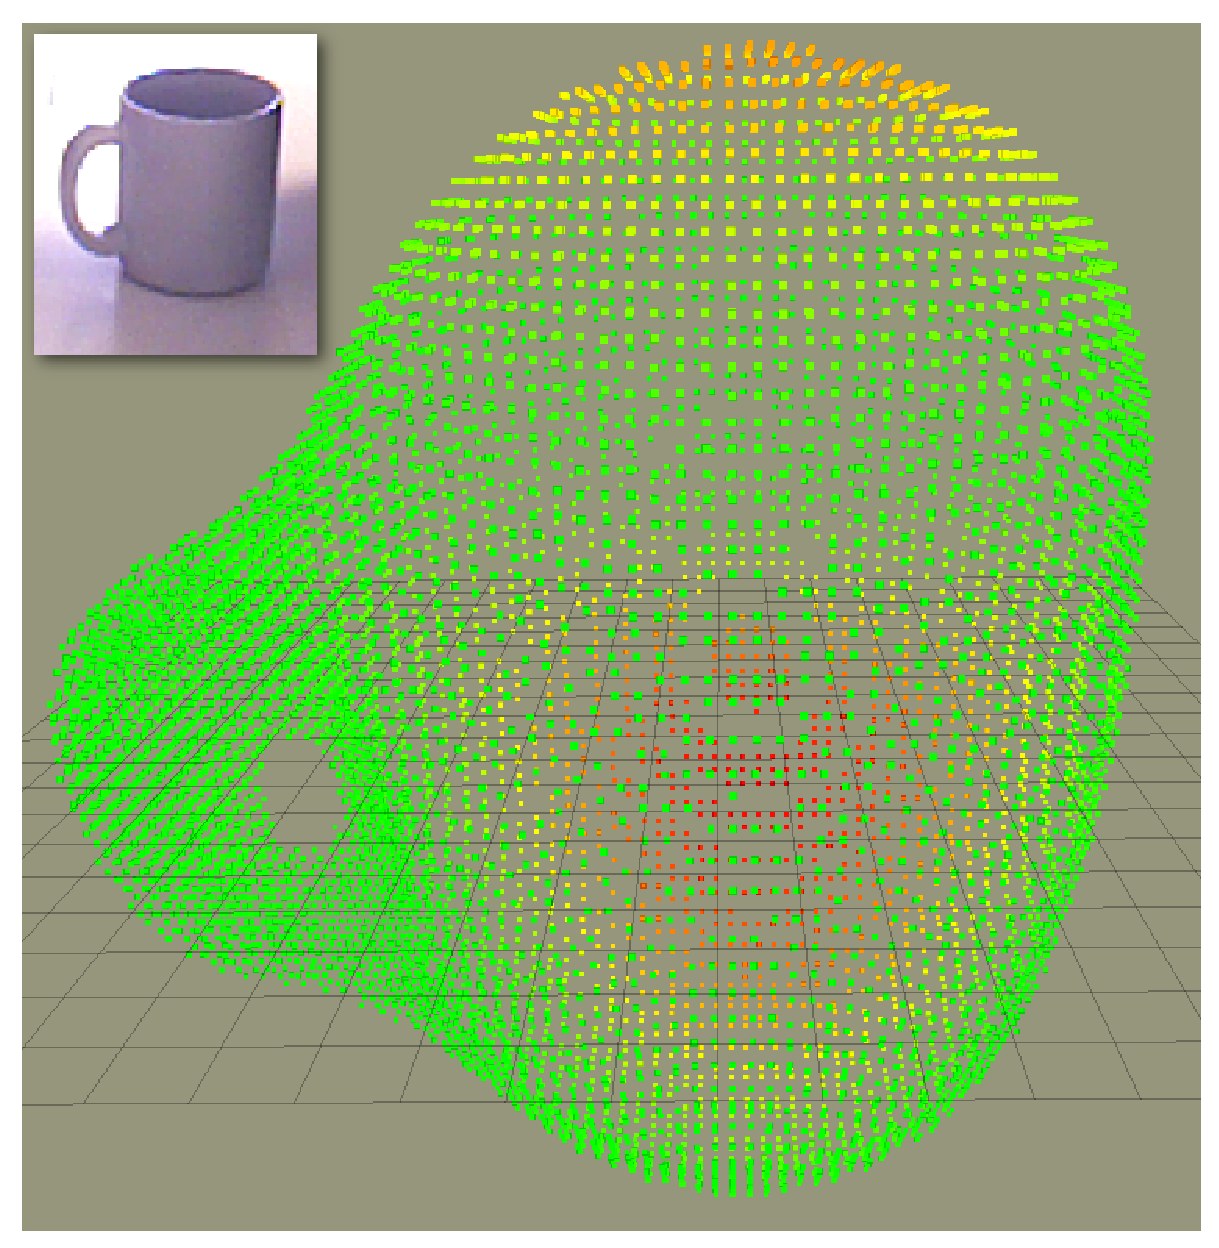
\includegraphics[width=0.6\columnwidth]{mugS.eps}
    \caption{Gaussian Implicit Surface, obtained from a mug (top-left corner) and sampled with a box-grid evaluation with fairly high point density. Each point has a predicted target $y_* \sim= 0$ and is colored accordingly to its associated
    predicted variance, from red (high variance) to green (low variance).}
    \label{fig:gpmug}
\end{figure}

A surface in 3D can be regarded as the $0$-level set of a family of surfaces defined by an implicit function $F(\mathbf{x}, y)=0$, where $F:\mathbb{R}^{3+1}\rightarrow \mathbb{R}$, with coordinates $\mathbf{x}\in \mathbb{R}^3$ and parameter $y\in \mathbb{R}$.
 Under the assumption that the Implicit Function Theorem holds, it can be expressed, at least locally, as $y = f(\mathbf{x})$, with $F(\mathbf{x},f(\mathbf{x}))=0$, and the surface of our interest raises when setting $y = 0$ --- the $0$-level set. Naturally, the value of $f$ (or $y$) increases to a positive value in outward normal direction to the surface ($\nabla F$), and decreases to a negative value in the inward direction ($-\nabla F$).

A Gaussian process (GP), on the other hand, ``is a collection of random variables, any finite number of which have a joint Gaussian distribution'' \cite[Def. 2.1]{Rasmussen2006Gaussian}, and it is completely specified by a mean, $m(\mathbf{x}) = \mathbb{E}[f(\mathbf{x})]$, and a covariance, $k(\mathbf{x},\mathbf{x}') = \mathbb{E}[(f(\mathbf{x}) - m(\mathbf{x}))(f(\mathbf{x}') - m(\mathbf{x}'))]$, function, where $\mathbb{E}(\cdot)$ is the expected value of a real process, such that we can write
\begin{equation}
f(\mathbf{x}) \sim \mathcal{GP}(m(\mathbf{x}), k(\mathbf{x},\mathbf{x}')).
\end{equation}

Now, let $\mathcal{S}$ be a set of tuples $s_i = (\mathbf{x}_i, \sigma_i, y_i)$ with $i=1,\ldots,n$, i.e. points, its corresponding noise characterization $\sigma_i$ and its target $y_i$, observed from a real process, one can in fact use the GP for regression for that training set, by specifying $m(\mathbf{x}=0)$, and a covariance function according to the nature of the process, to yield the model
\begin{equation}
\mathbf{y} \sim \mathcal{N}(\mathbf{0}, K(\mathcal{X},\mathcal{X}) + \boldsymbol{\sigma}^\top I \boldsymbol{\sigma}), \label{eq:gp_model}
\end{equation}
where $\mathcal{N}(\cdot, \cdot)$ denotes a normal distribution with mean and variance arguments, respectively, $\mathcal{X} \in \mathcal{S}$ the subset corresponding to the input space of the training set,  $K(\cdot, \cdot)$ the covariance matrix formed with elements $k_{ij} = k(\mathbf{x}_i, \mathbf{x}_j)$, for all $i,j : \mathbf{x}_i, \mathbf{x}_j \in \mathcal{X}$, and $\boldsymbol{\sigma}$ the $n$-vector corresponding to the noise characterization of the $i$th observation, therefore, $I$ is an identity matrix $n \times n$, and finally, $\mathbf{y}$ also the $n$-vector that collects the targets similarly. But the interesting part is the ability to predict a target, $y_*$, given a test input $\mathbf{x}_*$, where this expression can be block-expanded, respecting probability principles \cite{Rasmussen2006Gaussian}, to
\begin{equation}
    \begin{bmatrix} \mathbf{y} \\ \mathbf{y}_* \end{bmatrix} \sim
               \mathcal{N}\begin{pmatrix}\mathbf{0}, & \begin{bmatrix} K + \boldsymbol{\sigma}^{T} I \boldsymbol{\sigma}) &
                                                 K_* \\
                                                 K_*^\top &
                                                 K_{**} \end{bmatrix}
                           \end{pmatrix},
\end{equation}
where $\mathcal{X}_*$ is the set of test inputs, and $\mathbf{y}_*$ their corresponding predicted values by the trained GP model, arranged in the same $n$-vector fashion. For simplicity, we dropped the arguments of the matrices such that $K = K(\mathcal{X},\mathcal{X})$, $K_* = K(\mathcal{X},\mathcal{X}_*)$ and $K_{**} = K(\mathcal{X}_*,\mathcal{X}_*)$. Thus, the two  predictive equations can be derived from algebraic manipulation to
\begin{alignat}{2}
	\mathbf{y}_* = & K_*^\top [K + \boldsymbol{\sigma}^{T} I \boldsymbol{\sigma})]^{-1}\mathbf{y}, \label{eq:f_prediction}\\
	\mathbb{V}(\mathbf{y}_*) = & K_{**} - K_*^\top[K + \boldsymbol{\sigma}^{T} I \boldsymbol{\sigma})]^{-1} K_*. \label{eq:variance_f}
\end{alignat}

The covariance function specifies a distribution over functions with a notion of nearness among them, and it is a critical ingredient to select the appropriate one to get coherent predictions out of a GP model, a problem sometimes referred to as the \emph{kernel trick}. There is actually a full chapter dedicated to its study by \cite[see Ch. 4]{Rasmussen2006Gaussian}, however, none of them seem adequate for points belonging to an implicitly defined surface. \cite{Williams2007Gaussian} comes with the idea to use the thin-plate concept from data interpolation, and obtained good results for a surface in 3D with the covariance function
\begin{equation}
k(r) = 2r^{3} - 3Rr^2 + R^3,
\end{equation}
with the change of variables $r = \| \mathbf{x} - \mathbf{x}' \|_2$ using the $2$-norm as the distance between points, for clarity, and with $R$ being the largest $r$ that can be observed within the training set ---recall that this is a closed pointset in 3D taken from the object surface observations. In that case, the training set is noise-free, so besides adopting the same covariance function for our strategy, we also extend the training set to be the composition of points on the surface, $\mathcal{S}^0$, with tuples of the form $s_i = (\mathbf{x}_i, \sigma_i, 0)$, points outside the surface, $\mathcal{S}^+$, with tuples of the form $s_i = (\mathbf{x}_i, 0, +1)$ and points inside the surface, $\mathcal{S}^-$, with tuples of the form $s_i = (\mathbf{x}_i, 0, -1)$. Thus, the training set $\mathcal{S} = \mathcal{S}^0 \cup \mathcal{S}^+ \cup \mathcal{S}^-$, and its cardinality is the sum of the respective cardinalities. Without loss of generality, but a slight gain in efficiency and parameter tuning, we can work in a normalized and offset-free space, using as scale the larger distance and the centroid from the training set. This way, for instance, $R$ becomes a fixed parameter, as well as the $S^+$ and $S^-$ sets, a trick also exploited by \cite{Li2016Dexterous}. Of course, the model exploitation requires a re-scaling and re-centering processing step.

Up to this point, we are able to compute the expected predicted target $y_* = \bar{f}(\mathbf{x}_*)$ and the associated prediction variance $\mathbb{V}[f(\mathbf{x}_*)]$ for any given input in ambient space, namely $\mathbb{R}^3$ in our case, given a training set $\mathcal{S}$. This means that if we evaluate exhaustively a $3$-dimensional box-grid containing the implicitly defined surface, the points on the surface are those where $y_* \simeq 0$ with an associated variance. This is all we need to explore and compute efficiently candidate points on the surface that improve the overall variance of the predicted shape, and not with a complete rendering as the box-grid evaluation, or even a marching cube algorithm, that requires time.
As an example, Fig.~\ref{fig:gpmug} shows an implict Gaussian Process surface, sampled with a box-grid evaluation.

However, we must not forget that there is an actual probe going towards the candidate points, and probably the best direction to follow is that of the normal to the predicted surface at the candidate point, mostly to avoid local undesired collisions, so it would be handy to have also a prediction of that out of the same GP. In our case, the normal direction is actually parallel to the gradient of the function, a concept we will need in further sections as well. If we consider the posterior mean of the GP given in (\ref{eq:f_prediction}) for a single test point, we have
\begin{alignat}{2}
\bar{f}(\mathbf{x}_*) = & \mathbf{k}(\mathcal{X},\mathbf{x}_*)^\top [K + \boldsymbol{\sigma}^{T} I \boldsymbol{\sigma})]^{-1}\mathbf{y} \nonumber \\ = & \mathbf{k}(\mathcal{X},\mathbf{x}_*)^\top \boldsymbol{\alpha}.
\end{alignat}
Note that, the vector $\boldsymbol{\alpha}$ is constant for a given training set $\mathcal{S}$, whereas the vector $\mathbf{k}(\mathcal{X},\mathbf{x}_*)$ gathers the covariance values between the test point and the training set being the only term depending on the test point. Therefore, the  gradient evaluated at $\mathbf{x}_*$ is computed as
\begin{equation}
 \frac{\partial \bar{f}(\mathbf{x}_*)}{\partial \mathbf{x}_*} = \frac{\partial \mathbf{k}(\mathbf{x}_*,\mathcal{X})}{\partial \mathbf{x}_*} \boldsymbol{\alpha}, \label{eq:gradient_f}
\end{equation}
which boils down to evaluate for each combination of test and training point the derivative of the thin-plate covariance function, explicitly
\begin{alignat}{2}
  \frac{\partial k(r)}{ \partial r} \frac{\partial r}{ \partial \mathbf{x}_*} = & [6r (r - R)] \frac{\mathbf{x}_i - \mathbf{x}_*}{\| \mathbf{x}_i - \mathbf{x}_* \|_2} \nonumber \\ \frac{\partial k_*}{ \partial \mathbf{x}_*} = & 6(r - R) (\mathbf{x}_i - \mathbf{x}_*),
\end{alignat}
for all $i : \mathbf{x}_i \in \mathcal{X}$. Consequently, the normal at the the test point, $\mathbf{n}_*$, is obtained dividing the gradient by its magnitude.

%Let $\mathcal{S}$ be a training dataset of $N$ observations, $\mathcal{S}=\{(\mathbf{x}_i, y_i)|i=1,\dots,N\}$, where $\mathbf{x}_i\in\mathbb{R}^n$ denotes the $i^{th}$ input vectors and $y_i\in\mathbb{R}$ the associated scalar output or target.  We collect the $N$ inputs vectors in a $n\text{ x }N$ matrix $X$ and the output target in a $N\text{ x }1$ vector $\mathbf{y}$, so that we can rewrite the training dataset in a more compact way as $\mathcal{S}=(X,\mathbf{y})$. We are interested in making inference about the mapping function $f:\mathbb{R}^n\rightarrow\mathbb{R}$ between the input vectors and the targets. We assume a linear regression model
%\[
%y_i=f(\mathbf{x}_i)+\epsilon
%\]
%where $\epsilon\thicksim\mathcal{N}(0,\sigma_n^2)$ is an independent identically distributed Gaussian noise with zero-mean and variance $\sigma_n^2$,


%A Gaussian process framework for regression (GPR) is a common choice to approximate $f(\mathbf{x})$, in which the targets $y_i$ are assumed to be drawn from a zero-mean multi-variate Gaussian distribution with a covariance matrix which is a function of the input vectors. Therefore the output distribution can be written as
%\begin{eqnarray}
%\label{eq:gpr}
%(y_1,\dots,y_N|\mathbf{x}_1,\dots,\mathbf{x}_N)\thicksim\mathcal{N}(0,K(X,X)+\sigma_n^2I)
%\end{eqnarray}
%The covariance function expresses somehow the notion of nearness or similarity, for which points in the input space $\mathbb{R}^n$ that are close would likely produce similar outputs. The choice of a kernel is a crucial ingredient for a GP and a vast part of the literature has investigated this problem, sometimes referred as the \emph{kernel trick}. Following previous works on implicit surface estimations we chose the \emph{thin plate} kernel, which is defined as
%\begin{eqnarray}
%\label{eq:thinplate}
%K(\mathbf{x}_i,\mathbf{x}_j)=2\|\mathbf{x}_i-\mathbf{x}_j\|_2^3-3R\|\mathbf{x}_i-\mathbf{x}_j\|_2^2+R^3
%\end{eqnarray}
%where $\|\mathbf{a}\|_2=\sqrt{\mathbf{a}^\top\mathbf{a}}$ and $R=\max(\|\mathbf{x}_i-\mathbf{x}_j\|_2),\forall\mathbf{x}_i,\mathbf{x}_j\in\mathcal{S}$, is the largest pairwise distance between the input vectors in the training dataset $\mathcal{S}$. To improve the prediction performance of the GP with a thin plate kernel is useful to divide the training dataset in three disjointed subsets, namely $\mathcal{S}^0=\{(\mathbf{x}_i,y_i)\in\mathcal{S}|y_i=0\}$ are the inputs labelled as ``on the object's surface'', $\mathcal{S}^+=\{(\mathbf{x}_i,y_i)\in\mathcal{S}|y_i=+1\}$ and $\mathcal{S}^0=\{(\mathbf{x}_i,y_i)\in\mathcal{S}|y_i=-1\}$ are artificial inputs, respectively, laying outside and inside the object's surface. We then can rewrite the training dataset as $\mathcal{S}=\mathcal{S}^0\cup\mathcal{S}^+\cup\mathcal{S}^-$ and its cardinality $N=N^0+N^++N^-$ as the sum of the respective cardinalities.

%Given a new point $\mathbf{x}_*$, it is possible to query the GP to compute the estimate of $y_*=\bar{f}(\mathbf{x}_*)$ with a measure of confidence expressed by its associated variance $\mathbb{V}[y_*]$ by deriving the following equations from Eq.~\ref{eq:gpr}:

%\begin{eqnarray}
%\label{eq:gpr_mu}
%y_*=\mathbf{k}_*^\top(K+\sigma_n^2I)^{-1}\mathbf{y}
%\end{eqnarray}

%\begin{eqnarray}
%\label{eq:gpr_var}
%\mathbb{V}[y_*]=k(\mathbf{x}_*,\mathbf{x}_*)-\mathbf{k}_*^\top(K+\sigma_n^2I)^{-1}\mathbf{k}_*
%\end{eqnarray}
%Notice that we have introduced a more compact notation where, for a single query point $\mathbf{x}_*\in\mathbb{R}^n$, $\mathbf{k}_*=K(\mathbf{x}_*,X)$ is the $N\text{ x }1$ covariance vector between the query point and the training dataset $X$. Similarly, $K=K(X,X)$ is the covariance matrix evaluated on the training dataset and $k(\mathbf{x}_*,\mathbf{x}_*)$ is a scalar value denoting the variance between the query point and itself.

%\subsection{Gaussian process derivative}
%\label{sec:gpr_der}

% The gradient estimation can be computed using a mixed covariance function that takes as argument function values and partial derivatives of that function, that is,
% \begin{equation}
% k\left(f(\mathbf{x}), \frac{\partial f(\mathbf{x})}{\partial\mathbf{x}}\right)=\frac{\partial k(\mathbf{x}, \mathbf{x}')}{\partial\mathbf{x}}.
% \end{equation}



% In the previous section we introduced a general formulation of GPR to describes implicit surfaces in terms of its mean (Eq.~\ref{eq:gpr_mu}) and variance (Eq.~\ref{eq:gpr_var}). We also shown that, given an query input $\mathbf{x}_*$ it is possible to predict its expected target value, $\bar{f}(\mathbf{x}_*)$ as well as its associated expected variance $\mathbb{V}[f(\mathbf{x}_*)]$. As described in~\cite{Rasmussen2006Gaussian}, a GPR can be utilised to make prediction on the gradient of the approximating function, $\mathbb{E}[f'(\mathbf{x})]$. In the case of implicit surface this information is equivalent to make an estimate of the normal surface at the evaluated point $\mathbf{x}_*$.\todo[]{add citation here}

% The gradient estimation can be computed by using a mixed covariance function between function values and partial derivates. Given two input vectors $\mathbf{x}_i$ and $\mathbf{x}_j$ the mixed covariance function can be written as
% $$
% cov(f(\mathbf{x}_i), \frac{\partial f(\mathbf{x}_j)}{\partial\mathbf{x}})=\frac{\partial k(\mathbf{x}_i, \mathbf{x}_j)}{\partial\mathbf{x}_j}
% $$
% which is equivalent to calculate the vector of partial derivatives with respect to $\mathbf{x}_j$ of the original kernel function. The first partial derivate of the thin plate covariance can be written as
% \begin{eqnarray}
% \label{eq:gpr_der}
% \frac{\partial k(\mathbf{x}_i,\mathbf{x}_j)}{\partial\mathbf{x}_j}&=6(\mathbf{x}_i-\mathbf{x}_j)(\|\mathbf{x}_i-\mathbf{x}_j\|_2 + R)
% \end{eqnarray}

% For a single query point $\mathbf{x}_*$, we define
% $$
% \frac{\partial K_*}{\partial\mathbf{x}}=\frac{\partial\mathbf{k}(X,\mathbf{x})}{\partial\mathbf{x}}\bigg|_{\mathbf{x}=\mathbf{x}_*}
% $$
% as the $N\text{ x }n$ mixed covariance matrix between the function values at the training points $X$ and the partial derivatives evaluated at the query point.

% Therefore, similarly to Eq.\ref{eq:gpr_mu}, the expected normal, $\mathbf{n}_*$, on the query input $\mathbf{x}_*$ can be computed by the following equation

% \begin{eqnarray}
% \label{eq:gpr_n}
% \mathbf{n}_*=\mathbb{E}[f'(\mathbf{x})]=\frac{\partial K_*}{\partial\mathbf{x}}^\top(K+\sigma_n^2I)^{-1}\mathbf{y}
% \end{eqnarray}
% where $\mathbf{n}_*$ is a $n\text{ x }1$ vector.

%---------------------------------------
\subsection{Atlas of an implicitly-defined manifold}
\label{sec:atlas-rrt}

%Following the formulation in~\cite{Jaillet2013Path},

In general, it is not always possible to obtain a global parametrization of an implicitly defined manifold embedded in an ambient space. In our case, the manifold of attention is to be the surface of an object. \cite{Henderson1993COMPUTING} provides a precise method to compute the surface via a local parametrization that uses \emph{disks}. The concept is that a disk contains an exponential mapping, explicitly represented by a tangent basis at a domain point on the surface, and the size of the disks corresponds to the validity of that mapping. The disks are further projected onto the surface using a logarithmic mapping. The method typically starts with an initial point, $\mathbf{x} \in \mathbb{R}^3$, known to be on the surface, $f(\mathbf{x}) = 0$ (or very closed and projected onto it), and creates the first unbounded disk. From there, new disks are created, and carefully intersected with the previous ones to avoid getting into the same areas already covered, to create new disks and bound others. The method continues until there are no unbounded disks. These concepts have evolved into many applications, including the computation of constrained configuration spaces \cite{Porta2014CuikSuite}, and we now briefly describe it in a manner orientated to our use-case.

Let our implicitly defined manifold---or surface---be defined by the equality constraint $f$ as
\begin{equation}
\mathcal{X} = \{\mathbf{x} \in \mathbb{R}^3 : f(\mathbf{x}) = 0 \}.
\end{equation}
Then, for any arbitrary \emph{regular} point $\mathbf{x}_i \in \mathcal{X}$, we can find an orthonormal tangent basis, $\boldsymbol{\Phi}_i$, that satisfies
\begin{equation}
\begin{bmatrix} \nabla f(\mathbf{x}) \\ \boldsymbol{\Phi}_i^\top \end{bmatrix} \boldsymbol{\Phi}_i = \begin{bmatrix}  0 \\ I \end{bmatrix}, \label{eq:tangent_basis}
\end{equation}
Following the notation of \cite{Porta2014CuikSuite}, we are in the special case where $n=3$ and $k=2$, hence $I$ is the $2\times2$ identity matrix, and $\boldsymbol{\Phi}_i$ is a $3\times2$ matrix. This basis serves as an approximation of the commonly known exponential, $\mathbf{x}_j = \phi_i(\mathbf{u}_i)$, and logarithmic $\mathbf{u}_i = \phi_i^-1(\mathbf{x}_j)$, mappings, that satisfy the condition $\mathbf{x}_i = \phi_i(\mathbf{0})$, where $\mathbf{u}$ are the coordinates of a local parametrization of the manifold around the point $\mathbf{x}_i \in \mathcal{X}$. This bijective map is formally known as a chart $\mathcal{C}_i$ ---the former \emph{disks}. Then, in practice, a point in the parameter space, $\mathbf{u}_i$, is exponentially mapped using a two-step procedure. First, the point is transformed to the ambient space as
\begin{equation}
  \mathbf{x}_j^i = \mathbf{x}_i + \boldsymbol{\Phi}_i \mathbf{u}_i, \label{eq:tangent_approx}
\end{equation}
where the upper index is for tracking the current basis. Second, we solve the orthogonal projection defined by the system
\begin{equation}
\begin{cases}
f(\mathbf{x}_j) = 0,
\\
\boldsymbol{\Phi}^\top( \mathbf{x}_j - \mathbf{x}_j^i ) = 0,
\end{cases} \label{eq:projection}
\end{equation}
for instance, using a Newton procedure initialized at $\mathbf{x}_j = \mathbf{x}_j^i$, if no better guess is available. In our case, though, we project using a gradient descent like method. The validity region of a chart, in this context, is related to how safe it is to compute this mapping. Typical bounds are related to the local curvature and distance from the tangent space to the manifold. However, these features are not precisely known in our scenario, so this is one deviation from the exact chart creation, that will be described in the next section.

Thus, given a point $\mathbf{x}_i \in \mathcal{X}$, one can build a chart $\mathcal{C}_i$ that allows us to obtain a new point $\mathbf{x}_j \in \mathcal{X}$. Then, this new point can be used to generate a new chart $\mathcal{C}_j$, and so on. In order to avoid the parametrization of areas already covered by other charts, they are intersected according to their validity region, introducing the notion of bounded and unbounded charts, depending on whether they have been intersected from all directions or not. For instance, the initial chart is by definition unbounded. This coordination process yields the concept of an atlas $\mathcal{A}$: a collection of properly coordinated charts, that completely covers the manifold when there are no unbounded charts. Since we already differ on the validity region of each chart, we naturally also differ on their coordination.

Due to our assumptions at the beginning of the section, the manifold $\mathcal{X}$ is smooth everywhere, and we should not expect singularities either. The function, of course, exists for any point in the ambient space as $f:\mathbb{R}^3 \rightarrow \mathbb{R}$, as well as the tangent basis approximation of the exponential and logarithmic mapping, and related concepts.

Up to this point, we are able to compute an atlas $\mathcal{A}$ of an implicitly defined manifold ---again, or surface---, $\mathcal{X}$, given at least a point $\mathbf{x}_i \in \mathcal{X}$ (or very close to it so we can project it using the tangent basis approximation). However, nothing has been said about what would be the preferred direction from the initial chart $\mathcal{C}_i$ to expand. If we are computing the atlas exhaustively, we can choose randomly, since we are expecting to cover it all anyway. However, if one wishes to go from point $\mathbf{x}_i \in \mathcal{X}$ to point $\mathbf{x}_j \in \mathcal{X}$ always being in the manifold, perhaps there is no interest in computing the full atlas, but only the interesting part of the path that connects them. \cite{Jaillet2013Path} successfully combines the RRT technique with this idea of computing collision-free paths of constrained mechanisms. The main difference with our strategy is we configure the RRT for exploration of uncertain regions, that is, the atlas tends to go towards regions of the predicted surface that need to be improved via tactile exploration, which it is actually the goal RRTs were proposed for at first.

%In this work we aim to generate a path along an object surface, described as a manifold over a GP estimation, $\mathcal{F}$, that a robotic finger equipped with a F/T sensor can follow to gather new information about the shape of the object. Such an information will be then integrated in a probabilistic model (GP) in order to refine the manifold. The goal is to iteratively converge to a model of the object's shape in which the shape uncertainty becomes negligible.

%We build on the recent advances on sample-based techniques for asymptotically optimal exploration of a general manifold. Similarly to the work of~\cite{Jaillet2013Path} we use an RRT algorithm to construct a path on the manifold. However the major difference with their work is how we construct a chart around a given point $\mathbf{x}_i$ and how we select a new candidate node for the RRT algorithm.

%Given a point $(\mathbf{x}_i, y_i\in\mathcal{S}^0$ such that $y_i=0$ we compute its estimated normal, $n_i$, using Eq.~\ref{eq:gpr_n} and the chart $\mathcal{C}_i$ as a disc centred in $\mathbf{x}_i$ with radius
%$$
%\rho=\frac{1}{\mathbb{V}[f(\mathbf{x}_i)]}
%$$
%which is inversely proportional to the expected variance of our model at point $\mathbf{x}_i$. This allows us to construct larger tangent space in region in which the confidence of the model is higher and thus to reduce the allowed exploring region when the model has less information.

%From the chart $\mathcal{C}_i$ we can randomly sample a finite set of $d$ candidate parameter vectors $\mathbf{u}_p^i$ with $p\in[1,\dots,d]$. Each parameter vector $\mathbf{u}_p^i$ encodes a direction of exploration from the central point $\mathbf{x}_i$ to a point $\mathbf{x}_p^i$ such that
%$$
%\|\mathbf{x}_i-\mathbf{x}_p^i\|_2=\rho
%$$
%laying on the circumference of the chart. Using the exponential map described in Sec.~\ref{sec:atlas}, we compute the projection $\mathbf{x}_p=\psi_i(\mathbf{u}_p^i))$ such that $\mathbb{E}[f(\mathbf{x}_p)]\approx0$ which leads us to points that are estimated to be on the object surface by our probabilistic model. An user-defined threshold $\epsilon$ can be set to modify the system of equations in Eq.~\ref{eq:projection} to
%\begin{align}
%\label{eq:approxprojection}
%\begin{cases}
%|f'(\mathbf{x}_p)|&\leq\epsilon \\
%\Phi_i^\top(\mathbf{x}_p-\mathbf{x}_p^i)&=0
%\end{cases}
%\end{align}
%where $f'(\mathbf{x}_p)=\mathbb{E}[f(\mathbf{x}_p)]$ and $|\cdot|$ is the absolute value function.

%We then select the direction $\mathbf{u}_{p'}^i$ such that
%$$
%p'=\argmax_{p\in[1,\dots,d]}{\mathbb{V}[f(\psi_i(\mathbf{u}_p^i))]}
%$$
%to obtained a candidate target point $\mathbf{x}_{p'}$ ion the manifold.



%Moreover, this technique has been succesfully combined with RRTs to compute path on a constrained configuration space, more details can be found in .


%The GP for implicit function defined in Sec.~\ref{sec:gpr} defines a probabilistic representation of a unknown surface and therefore a global parametrisation of such a surface is not available. However we can interpret the surface as a manifold, $\mathcal{F}$, implicitly defined by a set of constraints such that $\mathcal{F}=\{\mathbf{x}\in\mathbb{R}^n|f(\mathbf{x})=0\}$. The manifold is represented as a collection of $k$-dimensional parameter spaces called charts.
%Given a point $\mathbf{x}_i\in\mathbb{R}^n$ on the manifold, a chart $\mathcal{C}_i$ is defined as a local parametrisation of the orthogonal tangent space at $\mathbf{x}_i$. We denote $\mathbf{u}_p^i\in\mathcal{C}_i$ a parameter vector such that
%\begin{equation}
%\label{eq:psi}
%\mathbf{x}_p^i=\mathbf{x}_i+\Phi_i\mathbf{u}_p^i
%\mathbf{x}_j^i=\pmb{\phi}_i(\mathbf{u}_j^i)=\mathbf{x}_i+\Phi_i\mathbf{u}_j^i
%\end{equation}
%where $\Phi_i\in\mathbb{R}^{n\text{x}k}$ is an orthogonal basis for the tangent space to the manifold at $\mathbf{x}_i$ and $\mathbf{x}_p^i\in\mathbb{R}^n$ is a point laying on this tangent space reachable from $\mathbf{x}_i$ through the parameter $\mathbf{u}_p^i$. Notice that both points $\mathbf{x}_i$ and $\mathbf{x}_p^i$ are defined in $\mathbb{R}^n$; in the literature this $n$-dimensional space is sometime referred as the ambient space (here a 3D space) to distinguish it from the $k$-dimensional space of the manifold (2D), with $n > k > 0$.

%To compute the tangent basis, $\Phi_i$, we make use of the estimated normal, $\mathbf{n}_i=\mathbb{E}[f'(\mathbf{x})]$, obtained by approximating the gradient of the GP at the point $\mathbf{x}_i$, as described in Sec.~\ref{sec:gpr_der}. Then we estimate $\Phi_i$ such that it satisfies the following linear system
%$$
%\left[
%\begin{array}{c}
%\mathbf{n}_i \\
%\Phi_i^\top
%\end{array}\right]\Phi_i
%=
%\left[
%\begin{array}{c}
%0 \\
%I
%\end{array}\right]
%$$
%where $I$ identifies the $k\text{ x }k$ identity matrix.

%The chart $\mathcal{C}_i$ also defines a bijective map between parameters $\mathbf{u}_p^i\in\mathbb{R}^k$ and $n$-dimensional points on the manifold. The function $\psi_i(\mathbf{u}_p^i)=\mathbf{x}_p$ is known in the literature as the \emph{exponential map} and defines the relation between the parameter space of the chart $\mathcal{C}_i$ and any point on the manifold $\mathbf{x}_p$. Similarly, the \emph{logarithmic map} expresses the inverse relation, $\psi_i^{-1}(\mathbf{x}_p)= \mathbf{u}_p^i$.

%A typical implementation of the exponential map makes use of Eq.~\ref{eq:psi} to move along the tangent space at $\mathbf{x}_i$ in the direction defined by the parameter vector $\mathbf{u}_p^i$, then it projects the point $\mathbf{x}_p^i$ on the object surface by solving the system of equations
%\begin{align}
%\label{eq:projection}
%\begin{cases}
%f(\mathbf{x}_p)&=0\\
%\Phi_i^\top(\mathbf{x}_p-\mathbf{x}_p^i)&=0
%\end{cases}
%\end{align}
%to find a point $\mathbf{x}_p$ that lays on the manifold and, therefore, on the estimated object surface.

%---------------------------------------
%\subsubsection{Implicitly-defined manifold exploration}
%\label{sec:AtlasRRT}


%%%%%%%%%%%%%%%%%%%%%%%%%%%%%%%%%%%%%%%%%
\subsection{Equipment specification and limitations}
\label{sec:limitations}

Tactile exploration requires a probe able to measure contact points on the surface of two rigid bodies, and preferably the normal at that contact point too. There are mainly two low-level sensor types suitable for this end: 1) tactile sensor arrays and 2) intrinsic tactile sensors\footnote{There are works reporting the use of a proprioceptive system, but we stick with these two.}. The first type is composed of a grid of pressure cells of fixed area, so the point resolution is limited to the quantization of the array. This kind of sensor has been widely used in the literature due to its multi-contact capability. However, in an scenario where a surface is not known precisely, it would require that the array be on top of a deformable body to exploit this feature most. But the deformation then becomes hard to measure, yielding useless point measures. Consequently, they are typically mounted on top of a quasi-rigid surface, also for safety of the cells, but in our scenario, we would be wasting the multi-contact capability. The second type is composed of a $6$-axis force-torque sensor and a known shape on top of it, typically one that allows the computation of the contact point and force in closed-form \cite{Bicchi1993Contact}. These are single-contact sensor with the resolution being that of the force-torque sensor measurement, which implicitly is the resolution of the A/D conversion of the internal load cells. This is, in general, smaller than the resolution of a tactile sensor array.

A consideration for both types is that, for tactile exploration, they need to be mounted on a robot with at least $6$ degrees of freedom, to allow the exploration to happen in different orientations w.r.t. the explored object. The mobility can be further increased if the object to be explored is also grasped by a movable robot with some degree of freedom. This inherently requires that the gripping device be soft and adaptive, but firm when grasping, since the initial assumption is that the shape is not known.

In both sensor types, the reachability space is of course limited to the size of the probe. It is worth considering, however, that with the intrinsic tactile sensor type, one can build a very small tip to reach tiny spaces.

% Object convexity concavity ?  Wait for Federico's feedback.

%%%%%%%%%%%%%%%%%%%%%%%%%%%%%%%%%%%%%%%%%
\subsection{Problem definition}
\label{sec:problem_definition}

Given all these ingredients, particularly that of having a probabilistic way to represent the surface of an object with a GP over initial and partial observations, the problem is: can we devise an exploration strategy \emph{intrinsic} to the model that exploits its probabilistic nature to suggest points\footnote{Note that the points can be isolated (poking) or arranged in a path (sliding).} for tactile exploration such that the predicted shape from the model improves? The following section provides details of our proposed solution, the GPAtlasRRT strategy.


%%%%%%%%%%%%%%%%%%%%%%%%%%%%%%%%%%%%%%%%%%%%%%%%%%%%%%%%%%%%%%%%%%%%%%%%%%%%%%%%
\section{GPAtlasRRT}
\label{sec:solution}

In the preceding section, we sketched how we relate Gaussian process implicit surfaces and the AtlasRRT methodology. The next paragraphs formally describe what we refer to as the GPAtlasRRT strategy. This strategy gives one possible answer to the question raised in the problem statement: it is a strategy that suggests local tactile exploration candidates to improve the object surface representation, exploiting its probabilistic nature. 

\begin{figure*}[t]
    \centering
    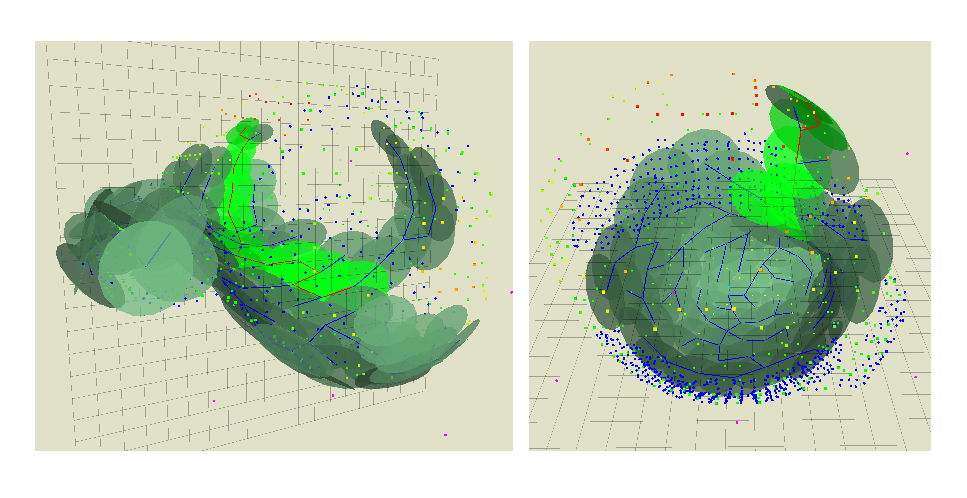
\includegraphics[width=0.95\linewidth]{twoAtlas.eps}
    \caption{The Atlas RRT expanding on implicit surfaces and highlighting the current next-best tactile action to perform. On the left the surface is estimated from a mug viewed from above. The mug is reported in the top-left corner. On the right the surface is from a circular container, also viewed from above.}
    \label{fig:GPAtlasRRTtwo}
\end{figure*}

The method starts from an initial and partial observation of the object surface. This is generally provided by a sensor such as a depth camera. To this end, we assume there is a way to segment the object from the background scene\footnote{We provide technical details of our approach in Subsection~\ref{sec:real}}. However, there might be no information at all, in which case the probe must naively move towards the palm of the gripper holding the object to obtain a first initial observation. As one would expect, the paucity of an initial shape estimate will increase the time to converge to an accurate shape. The initial observations form the set $\mathcal{S}^0$ to give the object surface model, $\mathcal{GP}$, model provided by (\ref{eq:gp_model}). Since these points are axiomatically on the surface with some degree of uncertainty due the sensor noise, we can compute charts on each of them.
Algorithm \ref{alg:strategy} describes the candidate points for tactile exploration to improve the input model, $\mathcal{GP}$, up to a predefined variance, $\mathbb{V}_{\max}$. 
The first step is to \textsc{selectSurfacePoint} (line \ref{init}) randomly to get a point $\mathbf{x}_i \in \mathcal{X} \subset \mathcal{S}^0$\footnote{In theory, we can start from all points in the surface, but in practice, this requires multiple processes to be properly synchronized.}. This is the starting point where the first chart is created, invoking the \textsc{createChart} function (line \ref{create_chart}). The generated data structure contains the center, $\mathbf{x}_i$, the orthonormal tangent basis provided by (\ref{eq:tangent_basis}), $\boldsymbol{\Phi}_i$, note that $\nabla f(\mathbf{x})$ is equivalent to (\ref{eq:gradient_f}), its size, $\rho_i$, and a set of points in the tangent space, $\mathcal{U}_i$. Two things are noticeable here that differentiate us from the original AtlasRRT algorithm. Firstly, the size of a chart, which is similar to the notion of a validity region, is inversely proportional to the variance at the chart center, namely,
\begin{equation}
\rho_i \propto \mathbb{V}[f(\mathbf{x}_i)]^{-1}.
\end{equation}
This size is actually the radius of a ball centred at $\mathbf{x}_i$, whose intersection with the tangent space yields \emph{disk}. The motivation behind this choice is that the more certain a point is to be on the surface, the larger the region of its chart on the predicted shape, whereas if more uncertainty is associated with the centre, smaller exploratory steps will be preferred. Second, a number of points proportional to the size of the chart are sampled from a random uniform density on an annulus of the disk with internal and external radius being $0.8\rho$ and $\rho$, respectively. The cardinality of this point-set in the tangent space is proportional to its size, namely,
\begin{equation}
\#\mathcal{U}_i \propto \rho_i.
\end{equation}
This leads to the fact that the larger the chart the more samples are needed to have a good quantization of it.
Another advantage of working with a normalized and offset-free set, as mentioned in Subsection \ref{sec:gpis}, is that the parameters that make the latter two expressions equal are tuned once, and remain fixed.

\begin{algorithm}[t]
    \textbf{$\mathcal{P} \leftarrow$ \textsc{GPAtlasRRT}}($\mathcal{M}$, $\mathbb{V}_{\max}$)\\ %functionname
\LinesNumbered
\DontPrintSemicolon
\SetAlgoVlined \SetKwInOut{Input}{input} \SetKwInOut{Output}{output}
\Input{A Gaussian Process model, $\mathcal{M}$ and the set of parameters $\Omega$, defining criteria
    to decide how to start, extend and end the exploration.}
\Output{The best next action, $\mathcal{P}$, in the form of a path, if any, or $\varnothing$ otherwise.}
$\mathbf{x_i} \leftarrow$ \textsc{selectSurfacePoint}($\mathcal{GP}$) \label{init} \\ 
$\mathcal{C}_{i} \leftarrow$\textsc{createChart}($\mathbf{x}_i$, $\mathcal{GP}$) \label{create_chart} \\
% $\mathcal{A}, \mathcal{T}, \mathbf{x}_{c,i} \leftarrow$\textsc{init}($\mathcal{M}$, $\Omega$) \\
$\mathcal{A} \leftarrow$ \textsc{addChart}($\mathcal{C}_i$) \label{add_chart} \\
  \label{is_expandable} \While{ \textsc{isExpandable}($\mathcal{A}$) }
  {
    $\mathcal{C}_j \leftarrow$\textsc{selectChart}($\mathcal{A}$) \label{select_chart} \\
    $\mathbf{x}_k \leftarrow$\textsc{expandChart}($\mathcal{C}_j$, $\mathcal{GP}$) \label{expand_chart} \\
    $\mathcal{C}_k \leftarrow$ \textsc{createChart}($\mathbf{x}_k$, $\mathcal{GP}$) \label{create_new_chart} \\
    $\mathcal{A} \leftarrow$\textsc{addChart}($\mathcal{A}$, $\mathcal{C}_k$) \label{add_new_chart} \\
    \label{ending} \If{ $\mathbb{V}[f(\mathbf{x}_k)]  > \mathbb{V}_{\max}$ }
    {
      $\mathcal{P} \leftarrow$ \textsc{getPath}($\mathcal{C}_i$, $\mathcal{C}_k$) \label{compute_path} \\
      \Return $\mathcal{P}$ \label{return_path} \\
    }
    % \textsc{connect}($\mathcal{T}$, $\mathcal{C}_{k}$, $\mathcal{C}_{j}$) \\
    %$\mathcal{C}_{i} = \mathcal{C}_{k}$ \\
  }
  %\eIf {\textsc{solution}($\mathcal{C}_{i}$)}
  %{\Return $\mathcal{P} \leftarrow$\textsc{path}($\mathcal{C}_{i}, \mathcal{T}$)}
  \Return $\varnothing$ \label{no_candidate}
  \caption{The GPAtlasRRT strategy} \label{alg:strategy}
\end{algorithm}


The algorithm continues with the addition of this first chart to the atlas, $\mathcal{A}$, that becomes the root node of an exploration tree (line \ref{add_chart}). The question whether an atlas \textsc{isExpandable} or not (line \ref{is_expandable}) is readily answered by checking whether there is at least one chart with $\#\mathcal{U}_j \neq 0$ or not. The \texttt{false} condition implies that we have completely covered the predicted surface, exiting with no candidate for tactile exploration (line \ref{no_candidate}). The \texttt{true} condition then makes the flow continue within the \textbf{while} loop for the iterative exploration. The first step is to \textsc{selectChart} (line \ref{select_chart}) to expand from the atlas. This action takes place randomly among all current charts whose point-set $\mathcal{U} \neq \emptyset$ using randomised selection between depth-first (selecting the previously expanded chart with probability $p = 0.4$) and breadth-first (selecting any other chart with probability $1-p$) for the tree expansion. Note that, in the first iteration, $\mathcal{C}_i$ is the only one, and it is surely expandable. Next, the \textsc{expandChart} operation on the selected chart (line \ref{expand_chart}) chooses among all points $\mathbf{u}_{j,t} \in \mathcal{U}_i$, the one with the largest variance in ambient space, that is,
\begin{equation}
\mathbf{u}_{j}^* =  \argmax_{\mathbf{u}_{j} \in \mathcal{U}} \mathbb{V}[f(\phi_j(\mathbf{u}_{j}))], 
\end{equation}
where the tangent basis approximation of the mapping $\phi_j(\cdot)$ is used as given in (\ref{eq:tangent_approx}). The point $\mathbf{x}_k^j = \phi(\mathbf{u}_{j}^*)$ is then projected to the predicted surface solving (\ref{eq:projection}), as mentioned, using a gradient-descent-like method to obtain the point $\mathbf{x}_k \in \mathcal{X}$. A chart, $\mathcal{C}_k$, is then created from this point and added to the current atlas (lines \ref{create_new_chart}--\ref{add_new_chart}). When a new chart is added to the atlas, the corresponding set $\mathcal{U}_j$ of all charts are reduced by discarding the points that fall within the validity region of the charts existing in the atlas according to our definition, that is, if they fall within the ball of radius $\rho_j$. This was not mentioned in the first call of the \textsc{addChart} in line \ref{add_chart}, because at that point there is only the root chart in the atlas. Finally, the expected variance of the center of the last chart added is compared against the input parameter $\mathbb{V}_{\max}$ (line \ref{ending}). The \texttt{false} condition of the \textbf{if} statement makes the algorithm continue with the atlas expansion, whereas the \texttt{true} condition returns the best exploration path, $\mathcal{P}$ (lines \ref{compute_path}--\ref{return_path}). Recall that this path is on the predicted shape of the object, therefore the control to follow it must be compliant to avoid damage. The new tactile observations tell whether the predicted shape is good or not by increasing the training set, $\mathcal{S}^0$, to automatically reduce the variance along the path, and improve the overall uncertainty of the surface model.
Figure~\ref{fig:GPAtlasRRTtwo}~and~\ref{fig:GPAtlasRRTfunnel} show the Atlas RRT expanding on various implict surfaces and finding the next-best tactile action to perform.
The next section describes how the GPAtlasRRT strategy can be embedded in a tactile exploration scenario.

\begin{figure*}[hbt]
    \centering
    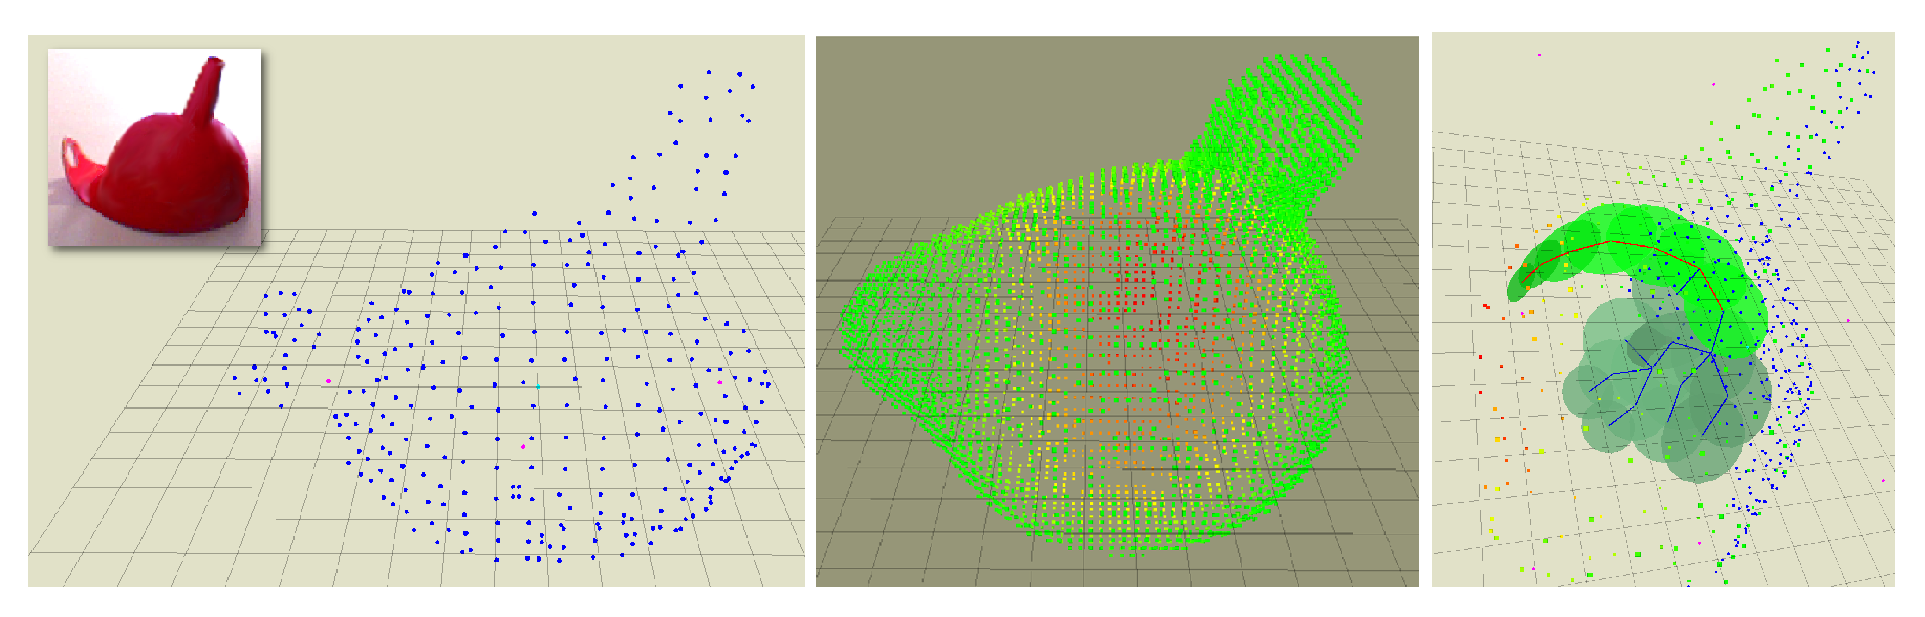
\includegraphics[width=0.95\linewidth]{funnel.eps}
    \caption{ A funnel (left-upper corner) is first seen by a depth camera. The segmented 3D points are shown in blue in the left figure to form the training set $\mathcal{S}^0$. The predicted shape by the GP on this set is shown in the middle obtained via a marching cube sampling algorithm. However, the GPAtlasRRT strategy does not require the explicit form of the predicted surface, as shown in the right figure. It works with the implicit form to devise the next-best tactile exploration shown in brighter green.}
    \label{fig:GPAtlasRRTfunnel}
\end{figure*}

\subsection{Tactile exploration for object surface modeling via the GPAtlasRRT strategy}
\label{sec:gpatlasrrt_tactile_exploration}

Algorithm~\ref{alg:solution} presents the pipeline model of a tactile exploration to model the surface of an object driven by the GPAtlasRRT strategy. As anticipated in the previous section, the initial and partial observation can be taken from visual input or a naive probe (lines to compute the model \ref{ini_gp}--\ref{fini_ini_gp}). From this point on, we plan the next-best tactile exploration, $\mathcal{P}$, (line \ref{exploration}), and pass this information to the exploratory probe. Please, note that this exploration can done by a real robot, or simulated given a ground truth, a notion that is used for the method validation in Section \ref{sec:experiments}.

It is worth noting, that in order to touch the object, this must be held such
that it does not move during the tactile exploration. But initially, the object
shape is not known. In a dual arm scenario, soft grippers that adapt locally to
the shape are ideal to tackle this situation. The issue is that their
adaptability makes it harder to sensorize, and it is difficult to measure how
they actually deform in order to segment an object when is being grasped by such
grippers. Thus, line~\ref{segment_object} is not as trivial as it seems. First of
all, we would need to define the gripper, which in our case is the Pisa/IIT
SoftHand~\cite{Catalano2014Adaptive}. This hand has been successfully sensorized
using IMUs~\cite{Santaera2015Lowcost} to recover the hand configuration.
With this information, along with the arm configuration, we are able to crop the
scene point cloud to focus on the hand-object cloud and to separate the
points belonging to the object and to the hand. The configuration
will be also useful for collision avoidance purposes during subsequent steps.
The fact that part of the object is covered by the hand limits the expandibility
of the GPAtlasRRT to estimate the complete object shape. To solve this, a
re-grasp manoeuvre is necessary, which is out of the scope of this work.

Thus, the exploratory probe system \textsc{approachTo} the exploration path, typically to the first point with low uncertainty when \emph{sliding} or to the final point with high uncertainty when \emph{poking} with the goal being a safe distance away from the predicted surface in the normal direction at the corresponding point. This phase can be executed with a position control scheme and collision avoidance motion planning. The latter is an interesting topic, since the object shape is not known. But it can be predicted with the current state of the model to some degree of uncertainty. A coarse point cloud can be computed out of the model and build a probabilistic collision map based on the expected variance of the function values at the point cloud. Next, we proceed to \textsc{probeObject} following the next-best path, $\mathcal{P}$, to get observations of points being on or outside of the surface, and labeled accordingly altogether in the exploration log set, $\mathcal{S}^{0+}$ (line \ref{probe}). In this phase, collision avoidance is disabled and the probe moves compliantly, as in a contour-following set-up, and uses the tactile sensing to detect whether the probe is in contact with the object surface. Once the end of the path is reached, the training set is updated accordingly, keeping the old training set and applying the normalization and offset-free operations after the addition of new data (line \ref{update_training}). This is then used to recompute a better model of the object surface, $\mathcal{GP}$ (line \ref{re-compute}). Simultaneously (using the old model) or afterwards (using the updated model), we engage again position control and collision avoidance motion planning to take the exploratory probe to its rest position (line \ref{away}). When the \textsc{GPAtlasRRT} returns an empty path, $\mathcal{P} = \varnothing$, then we say that the predicted shape by the returned model, $\mathcal{GP}$, has at most a variance of $\mathbb{V}_{\max}$ for any point on the surface, that is, $\mathbb{V}[f(\mathbf{x})] < \mathbb{V}_{\max}, \, \forall \mathbf{x} \in \mathcal{X}$. The next section presents two implementations of this algorithm, one that we use for validation, where the \textsc{probeObject} is performed by ray-casting on object meshes (ground truth), and another for testing, where our Vito robot is equipped with a tactile probe to execute this action.

\begin{algorithm}[t]
\textbf{\textsc{TactileExploration}}($\mathcal{Z}, \mathbb{V}_{\max})$\\ %functionname
\LinesNumbered
\DontPrintSemicolon
\SetAlgoVlined \SetKwInOut{Input}{input} \SetKwInOut{Output}{output}
\Input{An initial point cloud of the scene, $\mathcal{Z}$, and the desired variance, $\mathbb{V}_{\max}$, for the overall surface prediction.}
\Output{The object model as a Gaussian process, $\mathcal{GP}$.}
  \label{ini_gp} \If{ \textsc{isEmpty}($\mathcal{Z}$) }
  {
    $\mathcal{S}^0 \leftarrow $ \textsc{naiveProbe}() \\
  }
  \Else
  {
  \label{segment_object}  $\mathcal{S}^0 \leftarrow $ \textsc{segmentObject}($\mathcal{Z}$) \\
  }
  $\mathcal{S} \leftarrow$ \textsc{generateTrainSet}($\mathcal{S}^0$)
  $\mathcal{GP} \leftarrow $\textsc{computeModel}($\mathcal{S}$) \label{fini_ini_gp} \\
  \While { \texttt{true} } 
  {
    $\mathcal{P} \leftarrow $\textsc{GPAtlasRRT}($\mathcal{GP}, \mathbb{V}_{\max})$ \label{exploration} \\
    \If{ $\mathcal{P} \neq \varnothing$ }
    {
      \textsc{ApproachTo}($\mathcal{P}$, $\mathcal{GP}$) \label{approach} \\
      $\mathcal{S}^{0+} \leftarrow $\textsc{probeObject}($\mathcal{P}$) \label{probe} \\
      %$\mathcal{S}^0 \leftarrow$ \textsc{getOnSurface}($\tilde{\mathcal{S}^{0+}}$) \\
      %$\mathcal{S}^+ \leftarrow$ \textsc{getOutsideSurface}($\tilde{\mathcal{S}^{0+}}$) \\
      $\mathcal{S} \leftarrow$ \textsc{updateTrainSet($\mathcal{S}$, $\mathcal{S}^{0+}$)} \label{update_training} \\
      $\mathcal{GP} \leftarrow $\textsc{computeModel}($\mathcal{S}$) \label{re-compute} \\
      \textsc{MoveAway}($\mathcal{GP}$) \label{away} \\
    }
    \Else
    { 
      \Return {$\mathcal{GP}$} \label{solutionfound} \\
    }
  }
\caption{Surface modeling via GPAtlasRRT} \label{alg:solution}
\end{algorithm}

%\subsection{Probabilistic completeness}
%\label{sec:reasoning}

%First of all, we can safely assume that the surface of any household object is a $1$-component manifold.








% During the \textsc{ApproachTo} (line~\ref{approach}) (\textsc{MoveAway}, line~\ref{away}) phases, the robot uses position control and standard motion planning techniques with collision avoidance. Since we are modelling the shape, we need to ensure that everytime the robot moves close (away) from the object, it does not collide with the object. It is tentative to use the current estimated shape, but since we are not actually computing it explicitly in our approach, we choose the bounding sphere as the collision geometry of the object. Thus the robot moves towards (away from) the surface at the contact location in the normal direction until reaching the bounding sphere. After that, a standard motion planning is used to approach the object (get to the rest position).

% The \textsc{probeObject} (line~\ref{probe}) phase is engaged once the robot is within the bounding sphere. The robot uses Cartesian impedance control, with the Cartesian force, pose and impedance set properly for the given setup. These implementation details are given in the next section. Since we don't actually know where the surface is, we need to whether the robot actually touched something or not, in order to properly label the acquisition (lines~\ref{belonglabel} and~\ref{nobelonglabel}) 

% The method finishes when \textsc{exploreGPAtlasRRT} (line~\ref{exploration}) described in Algorithm~\ref{algo:strategy} has explore sufficiently the estimated shape and could not find an exploratory action $\Gamma$ (line~\ref{solutionfound}), i.e. the object shape is probabilistically estimated within the 95\% of the confidence interval computed from $\mathbb{V}_{des}$. 

%The complete solution of the problem as stated in~\ref{sec:scope} is depicted in Algorithm~\ref{alg:solution}.



%This section provides a more detailed description of our GPAtlasRRT algorithm. As described in Sec.~\ref{sec:scope}, our approach combines probabilistic inference on an unknown surface with a asymptotically optimal sample-based exploration technique for implicitly-defined configuration spaces (manifolds). We demonstrate the efficiency of our proposed solution in a bimanual framework (see Sec.~\ref{sec:scenario}) where a humanoid robot (Vito) can hold an unknown object in one hand and actively build up a probabilistic model of the object's shape by integrating visual and haptic information. This is done efficiently by selecting haptic actions which lead to an asymptotically optimal reduction of the global shape uncertainty of the model. 

%We employ a GP to learn a probabilistic model of the object surface, encoded as an implicit surface, constrained to visual and tactile clues iteratively acquired. First we rely on visual information captured by a RGB-D camera, which will be pre-processed, as described in Sec.~\ref{sec:segmentation}, to isolate the object's point cloud from the rest of the scene (robot's and environment's). Secondly we generate artificial points to improve the performance of the GP estimation, and after having labelled them properly we pass them as training inputs to the GP procedure. This procedure will be described in Sec.~\ref{sec:shape}. 

% The (noisy) visual observations constrain our model which has the effect of increasing its confidence (reduced variance) on its predictions about the function value $f(\mathbf{x})$ in regions highly populated by the training dataset. However, predictions in occluded or unseen regions will be associated with lower confidence (high uncertainty) since few or none information are available.  

% To improve the accuracy of our model, we make inference on it to build paths along the estimated object's surface such that a robot finger equipped with F/T sensors can collect haptic information over unseen regions of the surface. Since the surface is encoded as an implicit surface we need a more efficient way to make inference than to just attempt to reconstruct the expected object's shape via a highly-dense randomly generated samples. Instead we utilise the notion of manifold as a collection of local parametrisation (charts) such that we can make predictions on the neighbouring regions of already visited points as well as generate more charts on the more recent visited regions. To keep track of how the charts are generated and connected by themselves, we employ an RRT-like algorithm to build a tree of charts. The algorithm terminates when a path to a region, which is more promising to reduce the overall shape uncertainty of our model, is found.

%Section~\ref{sec:strategy} will explain the novelty of our algorithm in detail.  


% \begin{algorithm}[h]
% \textbf{\textsc{createGaussianProcess}}($X$)\\ %functionname
% \LinesNumbered
% \DontPrintSemicolon
% \SetAlgoVlined \SetKwInOut{Input}{input} \SetKwInOut{Output}{output}
% \Input{The training data, $\mathcal{X}$, in the form of a point cloud.}
% \Output{The Gaussian Process that models the object shape.}
%   $\mathcal{D} \leftarrow$\textsc{deMeanNormalizeAndLabel}(\{$\mathcal{X}$, $\mathbf{0}_{\text{sizeOf}(\mathcal{X})}$\}) \\
%   \textsc{addLabeledPoint}(\{$\mathbf{0}_3, -1\}$, $\mathcal{D}$) \\
%   \textsc{addLabeledPoints}(\{\textsc{sphere}$(\mathbf{0}_3, 1.1, N)$, $+\mathbf{1}_{N}\}$, $\mathcal{D}$) \\
%   $\mathcal{G} \leftarrow$ \textsc{doRegression}($\mathcal{D}$) \\
%   \Return $\mathcal{G}$ \\
% \caption{Gaussian Process regression} \label{algo:strategy}
% \end{algorithm}

%%%%%%%%%%%%%%%%%%%%%%%%%%%%%%%%%%%%%%%%
%\subsection{Best-next tactile strategy}
%\label{sec:strategy}

%Algorithm~\ref{alg:strategy} presents a pseudo-code of our implementation. As previously described in Sec.~\ref{sec:scope}, we explore the estimated surface of the object via a combination of probabilistic inference and sample-based techniques for manifolds. 

%We employ an RRT-like algorithm which, instead of growing in the ambient space, is embedded in an implicitly defined configuration space defined by a manifold or Atlas, $\mathcal{A}$. The major difference between our proposed implementation and a traditional RRT-algorithm is in how we select a new candidate node and expand the tree.


%
%The RRT explorer, however does not have any information on the model on which is built, specifically,
%it just need to track the connections between nodes of the tree and decide where it
%should expand next. All the model information is stored in an Atlas, called $\mathcal{A}$.
%
%An atlas can be viewed as a collection of maps or charts and conceptually it is able
%to create new charts at a given location on the surface it is currently modelling.
%Furthermore $\mathcal{A}$ is able to expand a given chart, producing new locations
%from where create new charts.
%
%In the proposed exploration strategy, RRT nodes are exactly the charts, thus
%building such a tree is like composing an atlas, which tries to model the implicit
%estimated surface.
%
%Formally we define a chart $\mathcal{C}$ with a center point on the surface $\mathbf{x}_{c}$,
%such that
%$$
%\mathbb{E}(\mathcal{S}(\mathbf{x}_c)) \approx 0
%$$
%with a search space defined as a
%tangent disc at the surface, centered on $\mathbf{x}_c$, with radius 
%$$
%R \propto \frac{1}{\mathbb{V}(\mathcal{S}(\mathbf{x}_c))}
%$$ 
%and finally with the gradient information at the center 
%$$
%G \approx \frac{\partial \mathcal{S}}{\partial \mathbf{x}}
%$$
%Conventionally the center variance is addressed as the chart variance, because
%it locally approximates the uncertainty of the surface estimation.
%
%With such charts, the atlas can be defined as the set of all charts plus some parameters
%responsible for chart creation:
%$$
%\mathcal{A} \triangleq \{\mathcal{C}_1, \ldots, \mathcal{C}_i, \ldots, \mathcal{C}_n, \Omega^{\mathcal{A}}\}
%$$
%where $n$ is the number of created charts and $\Omega^{\mathcal{A}}$ are the parameters.
%
%The explorer can also be viewed as a collection of chart connections, or branches,
%plus another set of parameters responsible for the tree expansion behaviour:
%$$
%\mathcal{T} \triangleq \{\mathcal{C}_i \leftarrow \mathcal{C}_j, \ldots, \Omega^{\mathcal{T}}\}_{i \neq j \le n}
%$$



%Given a Gaussian Process model, $\mathcal{M}$, approximating the implicit object surface
%with a regression, as described in Sec.~\ref{sec:gpr}, and the set of parameters
%$$\Omega \triangleq \Omega^{\mathcal{A}} \cup \Omega^{\mathcal{T}}$$
%An empty atlas and a RRT explorer can be initialized.
%Then a starting point is selected randomly among the object training set:
%$$
%\mathbf{x}_{c,i} \in \chi^0
%$$
%where $\chi^0$ is the set of object points,
%which in turn is part of the Gaussian Process Model, $\mathcal{M}$.
%
%$\mathcal{A}$ is charged to create the first chart, also called \emph{root}, from the starting point,
%then the algorithm rapidly builds the tree of charts on the object until the supplied termination
%criterion is met, or the maximum allowed number of charts has been reached.
%The best-next tactile action is finally the path from the converging chart to the root, or nothing if no such chart exists.

%The main loop of the algorithm is fulfilled by the following steps:\\
%\begin{inparadesc}
%\item[select($\cdot$)] Ask the explorer to select a chart to expand,
%among the chart collection ($\mathcal{A}$).
%This is done by selecting one at random with a bias to increase the probability
%of selecting the last created chart. This criterion is adopted to grow a tree
%which is more inclined to expand on a single branch, but at the same time maintain the
%possibility to create new branches from previous charts. So efficiency and speed
%is preserved, while we make sure we are exploring as much surface as possible,
%before reaching a solution.\\
%\item[expand($\cdot$)] The selected chart $\mathcal{C}_j$ is expanded by $\mathcal{A}$, by
%sampling $k$ points on its tangent discs then selecting one at maximum variance
%and at the same time not in collision with other charts search spaces. 
%So a sample $\mathbf{s}_i$ is selected if 
%$$
%\mathit{max}_{i\in k}[\mathbb{V}(\mathcal{S}(\mathbf{s}_i))]
%$$
%and 
%$$
%{\parallel\mathbf{s}_i - \mathbf{x}_{c,j}\parallel}_{2} > R_j, \forall \mathcal{C}_j \in \mathcal{A}_{i \ne j}
%$$
%where $\mathbf{x}_{c,j}$ is the center and $R_j$ is the tangent disc radius of $\mathcal{C}_j$.

%The selected $\mathbf{s}_i$ is then projected back on the surface,
%creating a center for a new chart, $\mathbf{x}_{c,k}$.
%The projection is performed with a gradient descend method, using the gradient estimation
%of the chart $G_j$.\\
%\item[create($\cdot$)] A new chart  is created on the projected point, maintaining the atlas
%    expansion on the estimated implicit surface
%$$
%\mathcal{C}_k \in \mathcal{A}
%$$
%\item[connect($\cdot$)] creates a connection to the chart which originated the newly created one,
%    drawing a new branch for the tree
%$$
%\{\mathcal{C}_j \leftarrow \mathcal{C}_k \} \in \mathcal{T}
%$$
%\end{inparadesc}

%$\mathcal{C}_k$ is then tested for the termination condition and the whole loop
%starts anew.

%The progressively growing tree of charts expands on the object surface until
%the termination criterion is met. Then, when this happens, the procedure terminates and the full
%path from the converging chart to the root of the tree is reported as a solution.

%Furthermore, to customize the exploration, the parameters in $\Omega^{\mathcal{A}}$ 
%control how much chart search spaces are big according to their variances and how many
%samples are generated during the \textsc{expand}($\cdot$) phase. 
%We chose to create tangent disc radii inversely proportional to their variance,
%because, when the uncertainty/variance is low, we want to expand further
%away from the starting chart, traversing reasonably certain surfaces faster.
%On the contrary, when the uncertainty/variance is high, we want to make small
%exploration steps, because we are not certain of the underlaying estimated surface.

%We chose to have a variance threshold as a termination condition, defined in $\Omega^{\mathcal{T}}$,
%because when the exploration reaches a chart with high variance, we want to stop
%the exploration and perform a tactile action there to reduce the uncertainty in the
%model. 
%% The action will bring new data to update the shape estimation and eventually 
% a new more accurate exploration can be started with updated model.


%%%%%%%%%%%%%%%%%%%%%%%%%%%%%%%%%%%%%%%%%%%%%%%%%%%%%%%%%%%%%%%%%%%%%%%%%%%%%%%%
\section{Experimental validation}
\label{sec:experiments}

%\subsection{Validation of the methodology}

% \subsection{Testing is simulated scenario}\label{sec:synth}
To validate the approach we first devised a simulation, where we performed tests on nine everyday objects, represented as polygonal meshes of (Figure~\ref{fig:meshes}).
\begin{figure}[t]
    \centering
    \includegraphics[width=0.95\columnwidth]{meshes-grey-scale-eps-converted-to.eps}
    \caption{Object meshes used as ground truth for our simulated tests. From top to bottom and from left to right: bowlA, bowlB, containerA, containerB, jug, kettle, spoon, mug and pot. The typical maximum dimension of each object is from 20-40cm.}
    \label{fig:meshes}
\end{figure}
These were obtained using an RGBD sensor and a turntable. They are used as ground truth and to create simulated depth images. Each trial iterated the \textsc{GPAtlasRRT} algorithm, Alg.~\ref{alg:strategy}~in~Sec.~\ref{sec:solution},
until the shape was predicted with desired variance $\mathbb{V}_{\max} = 0.1$.
% find a solution path that defines the best next tactile action to perform, until
The selected tactile actions were simulated using  raycasting. Rays are uniquely defined by a chart center, as pivot point, and its normal, as direction.
Thus we can define ray-mesh intersections as touches, and non intersections as points outside the surface. We adopted three different tactile schemes, thus forming three conditions, for a total of 27 full shape reconstructions. These are as follows.

\begin{asparadesc}
    \item[Random Touch] for the first condition the robot just attempted to touch a random point on the GP manifold. This repeated until the reconstructed shape had a maximum variance of $0.1$. This was our control condition or baseline. Test results are shown in Table~\ref{tab:tests}.
    
    \item[Single Poke] for the second condition we used the \textsc{GPAtlasRRT} by poking the last chart in the path. The convergence criterion was the same as for the random condition. Results in Table~\ref{tab:tests} show a significant reduction
 in the number of tactile actions required to reach the requested shape uncertainty.
 
    \item[Sliding Touch] for the  final condition we  used the full path generated by \textsc{GPAtlasRRT}. Starting from the root chart we made simulated touches and from each one re-interpolated the path toward the next chart. This was repeated until the tip of the atlas branch was reached. As the virtual probe moves across each chart many data points were gathered, in contrast to the single poke or random conditions. We hypothesized this condition would be the best performer in terms of the quality of the reconstructed shape, and in terms of the number of charts traversed. Table~\ref{tab:tests} shows this to be correct.
\end{asparadesc}
%\begin{table}
%    \centering
%    \begin{tabularx}{0.95\columnwidth}{lccccccr}
%        \toprule
%        Object &&& & & Steps && RMSE \\
%        \midrule
%        bowlA &&& & &67 && 0.0025\\
%        bowlB &&& & &38 && 0.0038\\
%        containerA &&&&& 124 && 0.0033\\
%        containerB &&&&& 68 && 0.0062\\
%        jug &&&&& 106 && 0.0027\\
%        kettle &&&&& 98 && 0.0031\\
%        spoon &&&&& 35 && 0.0058\\
%        mug &&&&& 238 && 0.0017\\
%        pot &&&&& 33 && 0.0035\\
%        \midrule
%        \textbf{Mean} &&&&& $\sim$\textbf{90} && \textbf{0.0036}\\
%        \bottomrule
%    \end{tabularx}
%    \caption{Random Touch test results in terms of the required number of actions (Steps) and the Root Mean Squared Error (RMSE) between
%    the predicted shape and the ground truth mesh.}
%    \label{tab:test1}
%\end{table}
%\begin{table}
%    \centering
%    \begin{tabularx}{0.95\columnwidth}{lccccccr}
%        \toprule
%        Object &&& & & Steps && RMSE \\
%        \midrule
%        bowlA &&& & &27 && 0.0023\\
%        bowlB &&& & &18 && 0.0036\\
%        containerA &&&&& 20 && 0.0035\\
%        containerB &&&&& 19 && 0.0043\\
%        jug &&&&& 20 && 0.003\\
%        kettle &&&&& 17 && 0.0032\\
%        spoon &&&&& 10 && 0.0055\\
%        mug &&&&& 28 && 0.0020\\
%        pot &&&&& 12 && 0.0032\\
%        \midrule
%        \textbf{Mean} &&&&& $\sim$\textbf{19} && \textbf{0.0034}\\
%        \bottomrule
%    \end{tabularx}
%    \caption{Single Poking test results in terms of the required
%    number of actions (Steps) and the Root Mean Squared Error (RMSE) between
%    the predicted shape and the ground truth mesh.}
%    \label{tab:test2}
%\end{table}
%\begin{table}
%    \centering
%    \begin{tabularx}{0.95\columnwidth}{lccccccr}
%        \toprule
%        Object & & &&& Steps && RMSE \\
%        \midrule
%        bowlA &&& & &8 && 0.0015\\
%        bowlB & &&& &5 && 0.0028\\
%        containerA &&&&& 11 && 0.0028\\
%        containerB &&&&& 8 && 0.0026\\
%        jug &&&&& 9 && 0.0025\\
%        kettle &&&&& 9 && 0.0029\\
%        spoon &&&&& 8 && 0.0031\\
%        mug &&&&& 12 && 0.0018\\
%        pot &&&&& 6 && 0.0028\\
%        \midrule
%        \textbf{Mean} &&&&& $\sim$\textbf{8} && \textbf{0.0025}\\
%        \bottomrule
%    \end{tabularx}
%    \caption{Sliding Touch test results in terms of the required
%    number of actions (Steps) and the Root Mean Squared Error (RMSE) between
%    the predicted shape and the ground truth mesh.}
%    \label{tab:test3}
%\end{table}

\begin{table}
    \centering
    \begin{tabular}{|l|c|r|c|r|c|r|} \hline
        & \multicolumn{2}{|c|}{Random Poke} & \multicolumn{2}{c|}{Single Poke} & \multicolumn{2}{c|}{Sliding}\\
        \hline
        Object & Steps & RMSE & Steps & RMSE & Steps & RMSE\\
        \hline
        bowlA & 67 & 0.0025 & 27 & 0.0023 &8 & 0.0015\\
        bowlB & 38 & 0.0038 &18 & 0.0036 & 5 & 0.0028\\
        containerA & 124 & 0.0033 & 20 & 0.0035 & 11 & 0.0028\\
        containerB & 68 & 0.0062 & 19 & 0.0043 & 8 & 0.0026\\
        jug & 106 & 0.0027 & 20 & 0.003 & 9 & 0.0025\\
        kettle & 98 & 0.0031 & 17 & 0.0032 & 9 & 0.0029\\
        spoon & 35 & 0.0058 & 10 & 0.0055 & 8 & 0.0031\\
        mug & 238 & 0.0017 & 28 & 0.0020 & 12 & 0.0018\\
        pot & 33 & 0.0035 & 12 & 0.0032 & 6 & 0.0028\\
        \hline
        \textbf{Mean} & $\sim$\textbf{90} & \textbf{0.0036} & $\sim$\textbf{19} & \textbf{0.0034} & $\sim$\textbf{8} & \textbf{0.0025}\\
        \hline
    \end{tabular}
    \caption{Simulated results for all three conditions in terms of the required number of actions (Steps) and the Root Mean Squared Error (RMSE) between the predicted shape and the ground truth mesh. RMSE is in meters.}
    \label{tab:tests}
\end{table}

The three experiments clearly show the superiority of the single poke and sliding touch methods in terms of number of required steps
and in terms of quality of the produced mesh. We performed Mann-Whitney tests to find the statistical significance of the difference between each pair of algorithms, by ranking their performances.\footnote{Despite not exploiting the paired nature of the data this is good test to use in the instance, as it avoids any assumptions about the underlying distribution of scores.}. For the number of separate touches until convergence all pairs of algorithms were significantly different at $p<0.001$ for a 2-tailed test. For the quality of implicit surface estimation the difference between the Sliding condition and the Single Poke was significant at $p<0.05$ for a 2-tailed test.

 As a final benchmark, Table~\ref{tab:comp} summarizes the comparison
between the test methods and Fig.~\ref{fig:shapecomp} shows some  of the \textsc{GPAtlasRRT} Sliding Touch reconstructed shapes with
the ground truth meshes next to them.\footnote{Additionally, we recorded videos of the shape reconstructions, see \texttt{goo.gl/4GKYTp}.}
\begin{table}
    \centering
    \begin{tabular}{|l|c|r|}
        \hline
        Tests  & Mean Steps & Mean RMSE \\
        \hline
        Random Touch & 90 & 0.0036\\
        Single Poking &19 & 0.0034\\
        Sliding Touch &8 & 0.0025\\
        \hline
    \end{tabular}
    \caption{Overall comparison: GPAtlasRRT with Sliding Touch outperforms in terms
    of efficiency and accuracy. RMSE is in meters.}
    \label{tab:comp}
\end{table}

\begin{figure}[htb]
    \centering
    \includegraphics[width=0.8\columnwidth]{comparison-grey-scale-eps-converted-to.eps}
    \caption{Comparison of reconstructed shapes (left) with the ground truth meshes (right), obtained with our GPAtlasRRT via the Sliding Touch method.}
    \label{fig:shapecomp}
\end{figure}


\subsection{Robot experiments}
\label{sec:vito}

\begin{figure}[htb]
    \centering
    \includegraphics[width=0.75\columnwidth]{Boris_jug002_crop-grey-scale.png}
    \caption{Real experimental setup. Boris explores an object fixed on the table.}
    \label{fig:boris}
\end{figure}

\begin{table}[t]
    \centering
    \begin{tabular}{c c c c c c} 
   	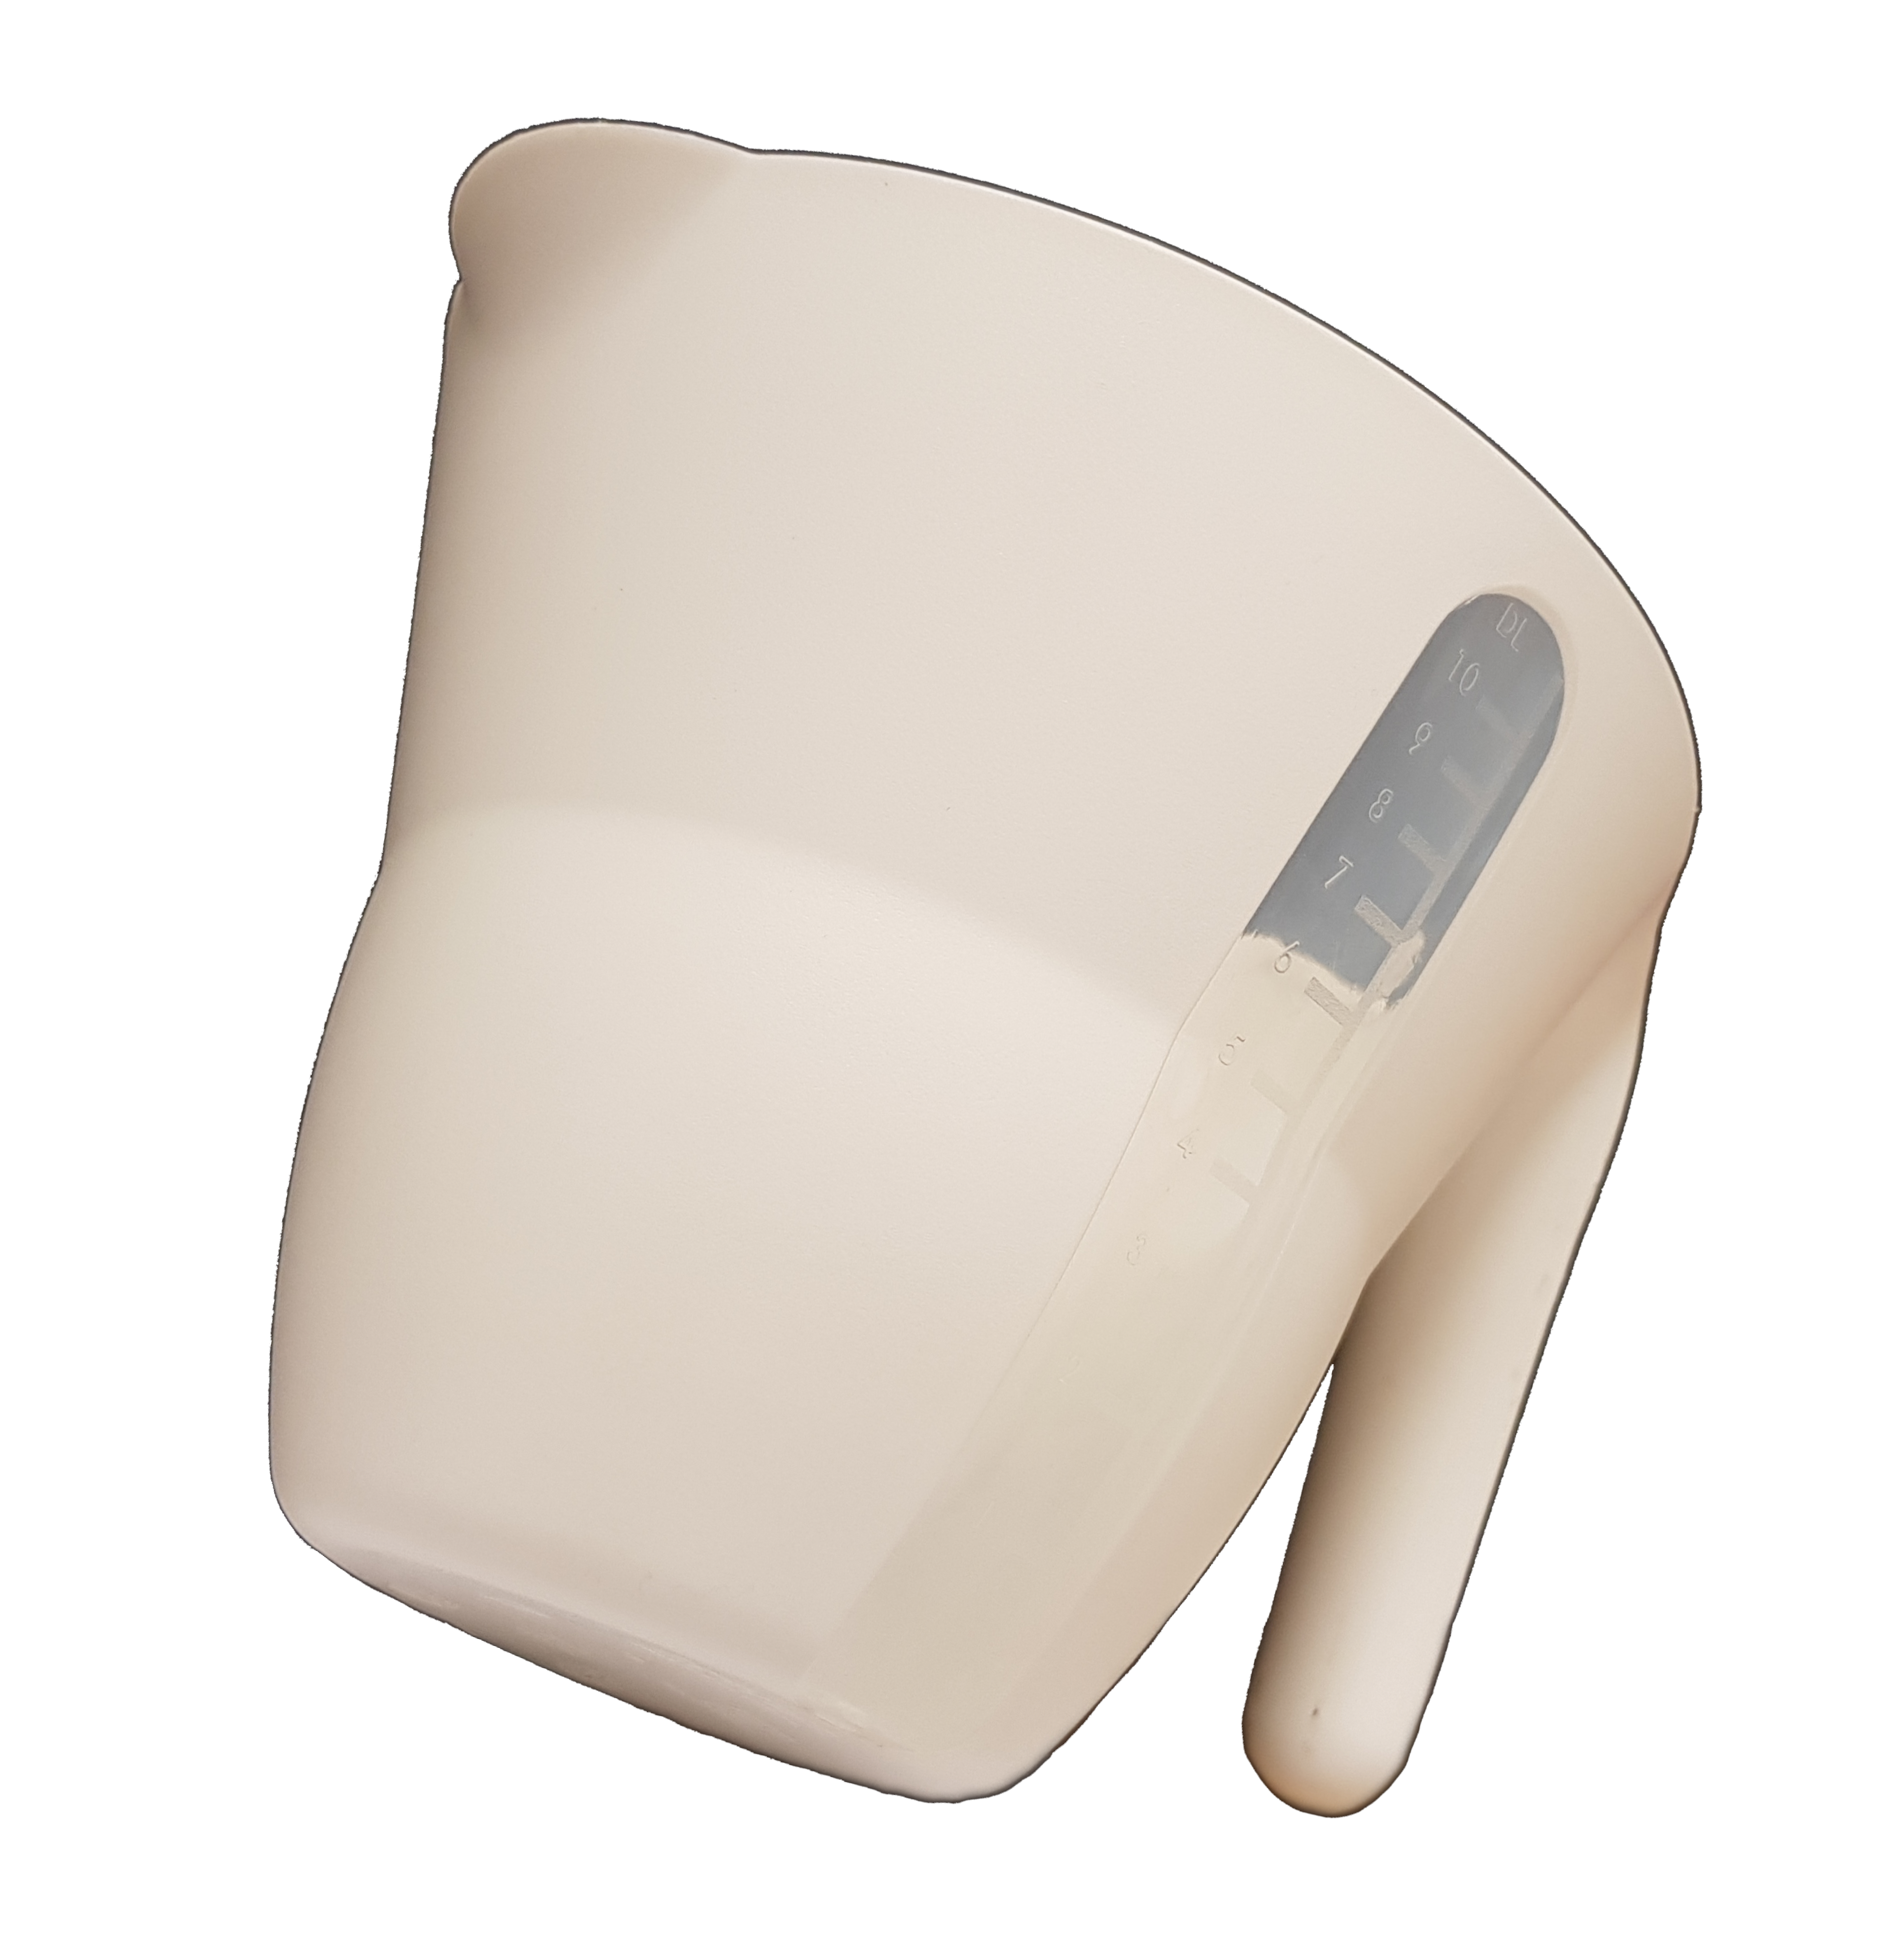
\includegraphics[width=0.12\columnwidth]{jug_white_1.png} &
    	\includegraphics[width=0.12\columnwidth]{jug_0_touches.png} &
	\includegraphics[width=0.12\columnwidth]{jug_5_touches.png} &
	\includegraphics[width=0.12\columnwidth]{jug_15_touches.png} &
	\includegraphics[width=0.12\columnwidth]{jug_25_touches.png} &
	\includegraphics[width=0.12\columnwidth]{jug_32_touches.png} \\
	\hline
       object &  (a) from vision & (b) 5 t & (c) 15 t & (d) 25 t & (e) 32 t \\
	\hline
        \end{tabular}
    \caption{Experiment on Boris. Left, the object and the initial GP model from the single view from the depth camera. The model improvement as the number of touches increases from left to right. The colours represent the variance from red (high variance) to blue (low variance). After fifteen touches the model already converges to the shape of the jug. The handle is excluded from inference since it is grasped and thus not explored. The GPAtlasRRT algorithm terminates after 32 touches.}
    \label{tab:boris}
\end{table}

This section provides an empirical evaluation of Algorithm \ref{alg:solution} on our real robotic platforms. As mentioned in Section~\ref{sec:gpatlasrrt_tactile_exploration}, we don't implement a re-grasping manoeuvre to overcome hand-induced occlusions, and thus reconstructions in the real robot case are incomplete, as we segment the grasped part of the object.\footnote{The implementation is mixed open-source \texttt{github.com/CentroEPiaggio/pacman-DR54}, heavily-based on the Robot Operating System \cite{ROS}. The GPAtlasRRT (Algorithm \ref{alg:strategy}) is a submodule \texttt{github.com/pacman-project/gaussian-object-modelling}. As with the simulated results, we present an accompanying video \texttt{https://goo.gl/4GKYTp}.} The technical details are now given.

In this scenario, we employ our Vito and Boris robots. These are bimanual robots equipped with 2 KUKA LWR 4+, one Pisa/IIT SoftHand~\cite{Catalano2014Adaptive} as one end-effector, and the intrinsic tactile sensor configuration as introduced by \cite{Rosales2014Active}. With Vito we start a trial by handing the robot an object. Afterwards, the object is segmented with the help of the recently developed IMU-based glove by \cite{Santaera2015Lowcost} to measure the hand configuration, and we remove the entire robot body from the scene. Other typical filters such as pass-through and down-sampling were applied to speed-up the overall pipeline. The acquired cloud contained an incomplete view of the object and constituted the initial training data for the Gaussian process, namely $\mathcal{S}^0$. Fig. \ref{fig:real} shows the initial model. Then a sequence of touches was performed. The experiments were performed using the single-poke condition.\footnote{The sliding condition requires more sophisticated impedance control than we had readily available. This makes sliding with our method a good piece of future work.} Planning for the bi-manual and unimanual set-ups used MoveIt. We performed both IK solving and path planning using this, and rejected tactile touches with unfeasible paths. In the event of path planning failure we simply restart the tactile exploration procedure.

The experimental results on Vito have shown that the grasping hand necessarily prevents full completion of the model, so an additional terminating condition is used.\footnote{This is a threshold for a number of failed consecutive attempts to execute a touch, and models the fact that it is not possible to touch areas occluded by the hand.} 
On Boris, the object is not handed to the robot, but held by a clamp. Thus we only used Boris's arm with the intrinsic tactile sensor. This choice was made so that---due to kinematic restrictions of this robot when operating bimanually without regrasp---the robot can reach and touch as large a proportion of the object's surface as possible, thus giving the most complete run of the tactile exploration algorithm. Figure~\ref{fig:boris} shows the setup.

On Boris we ran the tactile exploration algorithm on a white plastic jug. Table~\ref{tab:boris} shows the evolution of the estimated model against the number of touches. The colour of the points encodes the variance in the surface estimate, ranging from red (high-variance) to blue (low-variance). Table~\ref{tab:boris} (a) presents the initial model obtained from the point cloud. From left to right the models are generated after respectively 5 (b), 15 (c), 25 (d) and 32 (e) touches. It is interesting to see that even after 15 touches the model is already close to the final shape estimate for the jug, but the GP is uncertain and so the procedure keeps exploring until the variance is reduced to below the threshold everywhere. 


%The setup included three standard personal computers, where one was dedicated to the GPAtlasRRT strategy, one acted as the decision-maker and the last was the hardware server. Most time is consumed in the computation of the explicit form of the object for collision-avoidance motion planning. Suggested tactile actions were checked for an inverse kinematics solution. If this failed another touch candidate was requested. Note that both the GPAtlasRRT strategy and the motion planner are probabilistic, and their combination in some cases led to the planner being trapped in a local-minima.

\begin{figure}
\centering
%\mbox{
  \includegraphics[width=0.9\linewidth]{real_shots.png}
%}
\caption{Our Vito robot performs a tactile exploration action using the proposed GPAtlasRRT strategy. The per-point colour code  is the same as in Fig.~\ref{fig:setup_solution}}
\label{fig:real}
\end{figure}

%%%%%%%%%%%%%%%%%%%%%%%%%%%%%%%%%%%%%%%%%%%%%%%%%%%%%%%%%%%%%%%%%%%%%%%%%%%%%%%%
\section{Conclusions and future work}
\label{sec:conclusions}

This paper presented a method for exploring an object on all sides with a finger. Key to our approach was a combined shape representation and planning algorithm (GPAtlasRRT). The planner allows the robot to estimate the location of unseen and untouched surface. Together they allow planning of local tactile exploration of an incompletely modelled object. We demonstrated the benefits both in simulation, and on a real robot. The real robot system also demonstrated the ability to grasp an object with one hand, segment this hand from the object in an initial point cloud, and then extend the model with touches guided by GPAtlasRRT.

This local tactile planning strategy required bringing together Gaussian process implicit surfaces and the determination of implicitly-defined manifolds via continuation techniques. This exploited the ability of Gaussian processes to naturally represent model uncertainty. 

The beneficial features of the approach are several. First, the planning method does not require the computation of the explicit form of the entire predicted shape. Second, the strategy makes no assumptions about the exploratory probe. Third, it can plan sequences of tactile actions across a contiguous portion of the object surface, thus providing a detailed surface reconstruction. Fourth, the robot implementation allows the robot to explore an object as it holds it.

The proposed strategy was compared to a naive one, where touch rays were directed randomly. Our strategy outperforms this, whether using a single touch, or a touch sequence. The strategy was also tested successfully using our Vito and Boris robots. Previous published methods simplified the setting by placing the object on a table and then planning actions in a Cartesian space. This does not permit the robot to plan to traverse to the unseen back surfaces of objects with a single finger, or to explore objects rotated as they held in the hand. Instead, by creating an object centred representation, the method presented here is able to handle these cases, which are characteristic of human tactile exploration of objects.

Several points deserve further attention and future work. Perhaps most relevant to this work is the consideration of gradient observations as described by \cite{Solak2003Derivative}, especially due to our hardware setup. This feature has been presented in related work but not previously exploited. Another interesting point arises when discussing how to locally explore the model, that is, the direction to move within a chart. A third interesting topic is the use of the proposed strategy to drive a control loop where the controller command can be part of, or even just the first single step, of the exploratory path. According to our experience this is feasible and promising road to explore. Implementation issues also lead to non-trivial scientific problems. For example, the problem of maintaining a stable grasp during bi-manual exploration needs to be more thoroughly addressed. We found that an underactuated hand could maintain a firm hold of the object, but movements of the object in hand could seriously degrade the model quality. This could be addressed by re-estimating the object position in hand by best fitting its pose against the parts of the model that are most certain. The problem can also be addressed by carefully controlling the applied forces during exploration. We believe that position based planners are inadequate for this task, and that various compliant/force control strategies could be applied.


% The incorporation of other exploration primitives is also an interesting topic, that is, in our case we returned a path, but also dynamic aspects in the form of time-parametrized path (a trajectory) can yield other kind of information that can leave to a better model.

%%%%%%%%%%%%%%%%%%%%%%%%%%%%%%%%%%%%%%%%%%%%%%%%%%%%%%%%%%%%%%%%%%%%%%%%%%%%%%%%
\section*{Acknowledgements}
The authors would like to thank E. Farnioli for the fruitful discussions on Gaussian Processes, as well as to G. Santaera for the support with the IMU-based glove.

%\vspace{-2em}
%%%%%%%%%%%%%%%%%%%%%%%%%%%%%%%%%%%%%%%%%%%%%%%%%%%%%%%%%%%%%%%%%%%%%%%%%%%%%%%%
\bibliographystyle{plain}
\bibliography{bib/report,bib/marco}



%FIRST AUTHOR
%\vspace*{13pt}
%\noindent%
%\parbox{5truein}{
%\begin{minipage}[b]{1truein}
%\centerline{{\psfig{file=author1.eps,width=1in,height=1.25in}}}
%\end{minipage}
%\hfill         %to 2nd column
%\begin{minipage}[b]{3.85truein}
%{{\bf First-Author} received his/her M.S. and Ph.D. degrees from the\break 
%University of Name, in Year1 and Year2, respectively. From Year3
%to Year4, he/she was Researcher/Engineer/$\ldots$ at the\break
%Institute of Name, and worked on the project of Title. 
%From Year5, he/she was Associate Professor, and became full 
%Professor in Year6 at the University of Name. Now, he/she holds 
%Position at the Faculty of XXX of the University of Name. He/she\hfilneg}
%\end{minipage} } %close for parbox
%
%\vspace*{3.9pt}  
%\noindent
%is also the President/Director of Organization/Society.
%
%\hglue 15pt First-Author is the author of over X technical 
%publications, proceedings,\break
%editorials and books. His/her research
%interests include Mind topics, Body\break
%topics and Application topics (see IJHR's flyer). 
%He/she is the coordinator of the 
%collaborative research network on Humanoid Robots at the University of 
%Name, Country. He/she is an active member of the Y Societies, 
%and was the General Chair\break
%
%\vspace*{-12.3pt}  
%\noindent
%of Z Conferences in Country, and the Co-Chair of Z Conferences in Country.
%
%%SECOND AUTHOR
%\vspace*{13pt}  
%\noindent%
%\parbox{5truein}{
%\begin{minipage}[b]{1truein}
%\centerline{{\psfig{file=author2.eps,width=1in,height=1.25in}}}
%\end{minipage}
%\hfill %to 2nd column
%\begin{minipage}[b]{3.85truein}
%{{\bf Second-Author} received his/her M.S. degree in XXX
%Engineering from the University of Name, Country, and his/her
%Ph.D. degree in XXX Engineering from the University of Name,
%Country, in Year1 and Year2, respectively. From Year3 to Year4,
%he/she was at the University of Name, as Assistant/Associate/Full\break
%Professor. He/she is currently an Assistant/Associate/Full\break
%Professor in the Department of XXX, the University of Name,\hfilneg}
%\end{minipage} } %close for parbox
%
%\vspace*{4.8pt}  
%\noindent
%Country. From Year5 to Year6, he/she also served as
%Director/Manager/$\ldots$ with\break
%the Institute/Center/$\ldots$ of Name, where he/she was responsible 
%for research\break
%projects in the area of Topics.
%
%\hglue 15pt Second-Author is the author of over X technical
%publications. His/her research interests include Mind topics, Body
%topics and Application topics (see IJHR's flyer).
%
%\vfill\eject

\end{document}


